% 2026-10-08, later (interactive session, Claude Opus 5.5, per Leon: "In T17 can
%   you include the DOI refs for each paper"). Bibliography: the entries for T0 to
%   T16, T14a and T14b now end with each record's concept DOI (the all-versions
%   DOI, which resolves to the latest version), read from the Transport Papers
%   community on Zenodo the same day. T1's is its existing concept 21743863.
%   No other change; printed version stays 2.0. Recompiled: 29pp (unchanged),
%   0 errors, 4 overfull (unchanged, all above the bibliography), no undefined
%   references. verify_T17.py not re-run (no counted quantity touched).
% 2026-10-08 (interactive session, Claude Opus 5.5, per Leon: "provide a link to
%   the transport papers in the disclaimer ... for all v2.0 papers"). The
%   Authorship and disclosure paragraph now ends with one sentence giving the
%   Transport Papers community on Zenodo, as G01 gives it: "The papers of the
%   series are deposited in the Transport Papers community on Zenodo, \url{...}."
%   No other change; printed version stays 2.0. Recompiled: 29pp (unchanged), 0 errors,
%   4 overfull (unchanged), no undefined references. Script not re-run (no
%   computational content touched).
% 2026-10-07, later (per Leon: "update T17 to ensure page numbers are correct
%   etc"). Every page and check count in tab:status re-read against the current
%   PDFs and scripts after the day's G00, G01 and T14b changes: all twenty rows
%   correct as they stand (T0 to T16 by the audit, T14a 23pp/86 and T14b 36pp/60
%   by hand), no number changed. The bibitem for T14b now gives the films'
%   YouTube links (T14b carries them from today). Printed version stays 2.0.
% v2.0 (2026-10-07, derivation session, Claude Opus 5.5, per rule 20, at Leon's
%   request: "lastly update T17 and in the status table of the papers include
%   the up to date version numbers of the papers"; T12, T13, T15 at v2.0, all
%   affected papers at 2.0). Printed version 1.1 -> 2.0 (\date), per Leon. No
%   label added or changed; no numbered table row added or removed.
%   tab:status: a version column ("Ver.", the version on each paper's title
%   page: T1 3.0; T12, T13, T14, T15, T17 2.0; the rest 1.0), the payload and
%   remainder columns narrowed and the table set in \small with tabcolsep 4pt
%   (as the other tables are small) so that it fits the text width, which it
%   did not before (the old table overran by 21pt); "companion;" in T0's tier
%   cell given a break point (a pre-existing overfull box); the introducing sentence
%   and caption name it. T12 row: the proton condition, the Pati-Salam route
%   with U(1)_X, M_U 3.4e16, the weak angle an input fitted without tuning on
%   the registered 2-3 mixing route; remainder + the intermediate scale and the
%   grade-three coupling (T12 successor problems (7), (8)). T13 row: "the one
%   direction carrying the factor on a single family"; 28pp; remainder + the
%   grade-three coupling. T15 row: the valuation at both ends, T12's route
%   selecting the bottom-like one; 22pp/53; remainder + the branch on T12's
%   route. Series total 1759 -> 1762 at all five body sites (T15 50 -> 53).
%   tab:refutations row 14: the running must change, through partner-like
%   content (no other tower supplies it) or an intermediate symmetry (Pati-
%   Salam from the slot/pair split, the weak angle then an input).
%   tab:directions row 10: the proton condition, the second route, the
%   registered 2-3 mixing route; remaining + the intermediate scale and the
%   grade-three coupling.
%   sec:verification: "seventy-four" -> "seventy-five"; Part A "forty-six" ->
%   "forty-seven", with the version check named.
%   verify_T17.py v2.0: the status-row parser reads the new column; recorded
%   T13 pages 27 -> 28, T15 50 -> 53 checks and 21 -> 22 pages, total 1759 ->
%   1762; NEW check A12, every version in the table equal to the version the
%   paper's own title page prints (twenty papers, T14a and T14b included,
%   this paper's own row read from its own \date).
%   Compile: pdflatex x3, 29 pages (28 before), 0 errors, 0 undefined refs, 0
%   multiply defined, 4 overfull boxes (the stance table's three and Part D's
%   one, pre-existing; the status table's four pre-existing ones are gone).
%   Audit: verify_T17.py 75/75 PASS, 0 skipped, in the cloud workspace against
%   the seventeen companions compiled there (A5.T13 28, A5.T15 22, A6.T15 53,
%   A12 20 rows). Em dashes: 0. Cross-references (rule 21): verify_crossrefs.py
%   T17 5/5 both directions; suite sweep 740 locators, 738 ok; the two failures are pre-existing and outside
%   this pass (T14a line 670, \cite[Premise P2]{ButlerT14}).
% v1.3 (2026-10-07, mechanical pass, per Leon: "Please perform the mechanical
%   pass" for T12 v1.1, whose header lists T17's status row and verify_T17.py's
%   pages dict among the knock-ons for that pass). Data refresh on the 2026-10-05
%   precedent; no mathematics, no label and no prose changed. tab:status T12
%   64pp/206 -> 75pp/243 (T12 v1.1: the proton condition, the slot/pair split and
%   the weak angle on the Pati-Salam route). Series total 1722 -> 1759 at all five
%   body sites. verify_T17.py: recorded T12 count 206 -> 243 and pages 64 -> 75,
%   total 1722 -> 1759 (A4 and the docstring), comment refreshed.
%   NOT done here (content, for a derivation session): the T12 row's payload, which
%   still summarises v1.0 (the supersymmetric row "admissible at two loops", no
%   proton condition, no Pati-Salam route, sin^2 theta_W = 3/8 with the angle not
%   yet marked an input on that route); refutation row 14, whose corrected
%   statement should name both routes; the matter-programme reading (the two-term
%   structure cannot reach the angle without tuning).
%   Compile: pdflatex x3, 28 pages, 0 errors, 0 undefined refs, 0 multiply defined,
%   8 overfull boxes (the pre-existing eight, none new). Audit: verify_T17.py 74/74
%   PASS, 0 skipped, run in the cloud workspace against the suite's seventeen
%   companion PDFs and headers (A5.T12 75 pages; A6.T12 243, form N/N; A4 1759).
% v1.2 (2026-10-05, mechanical pass, per Leon: "update T17 as part of the
%   mechanical pass"). Data refresh after T14 v2.0, on the precedent of the
%   2026-09-11 pre-flight; no mathematics and no label changed. tab:status T14
%   50pp/94 -> 74pp/200 (T14 v2.0: the unit-ball rule, Section 7; Part N's two
%   floating-point checks added 2026-10-05), and one clause in its payload
%   naming the unit-ball rule (fitted, observation level, floor 5.255) and the
%   cluster result (passes only with the odd towers' matter collisionless, a
%   premise). Series total 1616 -> 1722 at all five body sites. New row after
%   T14a for the companion T14b ("Simulating the Dark Towers", 36pp, 60 checks;
%   formerly numbered T14c; the earlier odd-towers note once numbered T14b is
%   T14z, outside the series and still not referenced), per Leon's 2026-10-02
%   instruction that T14b appear in the series tables; outside A3's row regex,
%   like T14a's, and not in the total. Section 3's companion clause and the
%   Position section name T14b; bibitem ButlerT14b. verify_T17.py: recorded T14
%   count 94 -> 200 and pages 50 -> 74, total 1616 -> 1722, comment refreshed.
% T17 of the Transport Papers series (the capstone; the last paper).
% v1.1 (2026-09-18, per Leon: the companion note T14a (One Dimension at a
%   Time: The Odd Extensions of the Oriented Towers) enters the capstone; the
%   other companion, T14b (Twistors in Odd Dimension and the Odd Towers), is
%   numbered in the suite but, at Leon's instruction later the same day, NOT
%   referenced here: its row, bibitem and Position mention were removed after
%   a first pass had added them; no other paper touched).
%   Insertions only, no renumbering: one row in tab:status after T14 (T14a
%   23pp, 86 checks; the row is outside verify_T17.py's A3 audit, whose row
%   regex and recorded dicts cover T0..T16 only, and is not counted in the
%   1616 series total); one clause
%   in the Section 3 opening sentence; one clause in tab:directions row 8
%   and one sentence in sec:measure (T14a's Theorem 8.2: the transport
%   constrains the frozen point only through its norm); the Position section
%   lists T14a after T14; bibitem ButlerT14a. No locator into the companion
%   is used (paper-level citation only).
%   verify_T17.py re-run in the cloud workspace: unchanged (39 run, 35
%   skipped for absent companion PDFs, 0 failed). Compile: pdflatex x3,
%   27 pages (was 26), 0 errors, 0 undefined references; 8 overfull boxes in
%   the two longtables' narrow columns, all present in v1.0's build and none
%   new.
% REVIEWED & DONE per Leon, 2026-09-11, the eighteenth and last paper declared
%   done. Numbering FROZEN at this version per rule 21. verify_crossrefs.py T17
%   run at declare-done in the cloud workspace against freshly compiled .aux
%   files of all eighteen papers: 5 locators checked, 5 ok, both directions;
%   the suite sweep (--all) 599/599, 0 skipped. verify_T17.py 74/74. No text
%   change in this entry; header only, recompiled so the PDF postdates the
%   source: 26 pages, 0 errors, 0 undefined refs.
% Zenodo pre-flight (2026-09-11, Fable 5.1, per Leon: all pre-flight fixes).
%   Reconciliation against the current siblings, caught by this paper's own
%   audit (5 of 72 failing): tab:status T1 50pp -> 51pp (Lean kernel
%   paragraph, 2026-09-10); T14 48pp/95 -> 50pp/94 (v1.3 mirror-share
%   derivation); T16 29pp/143 -> 31pp/146 (v1.2 plain description). Series
%   total 1614 -> 1616 at all five body sites (abstract, Sec 3 method, Sec 5
%   preamble, tab:status caption, Sec 8 Part A). verify_T17.py: recorded
%   counts and pages tables refreshed to match, total 1614 -> 1616; T0's
%   header now records its 16/16 re-run so A6.T0 no longer skips. Audit
%   re-run in the cloud workspace against the recompiled siblings: 74/74,
%   0 skipped. No other text, label or number changed; newlabel diff is the
%   tab:status caption only.
%   Compile: pdflatex x2, 26 pages, 0 errors, 0 undefined refs, 8 overfull,
%   152 underfull (both unchanged), no float overflow.
% Terminology (2026-09-11, per Leon): "pencil" retired in the body, matching
%   T16's rename to the incidence-line phrasing. tab:status T16 row: "every
%   point a pencil of vacua and spacetime the manifold of pencils" -> "every
%   point a projective line of vacua and spacetime the manifold of such
%   lines", and "the pencil picture's exhaustiveness" -> "the incidence-line
%   picture's exhaustiveness". Section 5 closing paragraph: "a pencil of
%   quantum vacua" -> "a projective line of quantum vacua". 4 replacements.
%   No mathematics changed and no label changed. Header entries above are left
%   as written.
%   Compile: pdflatex x2, 26 pages, 0 errors, 0 undefined refs, 8 overfull and
%   152 underfull, every one pre-existing and unchanged in count from v1.1.
% Correction (2026-09-10, mechanical pass, per Leon): rule 23 misidentified T5 as the printed-version exception. T1 is the exception at Version 3.0; every other paper, T5 included, reads Version 1.0. \date corrected accordingly (was 1.1).
% v1.1 (2026-09-10, derivation session, Fable 5.1 subagent, per rule 20,
%   series-review repair pass against series_review_2026-09-09.md).
%   Reconciliation after the sibling repairs (same session): status-table
%   page counts T5 76pp -> 77pp (Position section added at v3.1) and
%   T6 30pp -> 31pp (Fact 6.10 split, Luk-Oh bibitems, v1.1); check counts
%   unchanged for every paper, series total 1614 unchanged.
%   2.1: T11 row of tab:status rewritten to T11 v-current: dictionary with
%   the minus sign, m^2 = -w(w+3)<I,I> = -w(w+3)Lambda/3 (T11 Thm 3.1), the
%   de Sitter reading, the join as the grip with the Lambda/3 correction, the
%   massless locus; "candidate (A)", "five constants with one equation",
%   "(oscillator Casimir)" removed; remainder = T11's five successor
%   problems. Refutation row 5 restated per T11 rem:hierarchy (imaginary
%   parts of the weights). Direction 10: "five constants of the exact join
%   (one equation in hand)" -> the operator join and the many-twistor grip.
%   sec:verification Part D: "-w(w+3)Lambda/3" with the sign checks named.
%   2.2: T14 row: "five against 5.364 with the GeV mean mass" removed; five
%   is the count of dark causal residues under P3, Omega_dark/Omega_b =
%   1 + 4.364, remainder symmetric and not derived. Part C description
%   rewritten to the ratio arithmetic T14 still does. Stance 9: conditional
%   as T14:1244 registers it. Stance 11: six populated, five dark, dimming of
%   order the tower count if comparable, dof counts not derived.
%   2.3: stance 6 "per quarter horizon cell" -> "per four Planck cells of
%   horizon area" (T8 Cor 4.4(2)); kappa_c for the calibration residue in
%   stance 6, the T8 row, and directions 2 and 4 (T8 Prop 4.12 keeps kappa_c
%   distinct from the surface gravity kappa).
%   2.11: sec:tiers: the tier is recorded where a paper declares it (abstract
%   or introduction) and is this survey's assignment otherwise.
%   2.12: T2 row: kinematic-singularity reading attributed to this paper's
%   sec:thesis remark, not to T2; refutation 13: "between forty-four and one
%   hundred and five orders" (T13:487).
%   Section 3: sec:intro "always and provably" scoped to T1 thm:nogo
%   (isotropic vectors, mixed signature, n >= 3; hyperbolic plane excepted;
%   type P needs no repair); T15 row: rank one at leading order whatever
%   alpha, the branch alpha << M_3 a separate premise; sec:houserules "T5 was
%   revised once" dropped (rule 17); T4 row remainder matched to T4's own
%   open list (Kasner-weights conjecture beyond the diagonal class, Kerr,
%   operator/state level, variable-exponent limit, edge regularity, twisted
%   completion); direction 4 "no longer waits" -> "does not wait".
%   Rule 18: sec:position added as Section 9 after Machine verification (no
%   sibling cites a T17 section number; Tables 1 and 4 keep their numbers).
%   T2 bibitem subtitle -> "and Where PGA's Missing Division Goes". Date
%   line Version 1.1. Status-table page and check counts of the other papers
%   NOT touched (coordinator reconciles after the sibling repairs land).
%   Script: verify_T17.py 74 checks, count unchanged (A 46, B 4, C 5, D 9,
%   E 7, F 3). C3-C5 replaced by T14's ratio arithmetic (4.364 = 5.364 - 1;
%   0.0976 +- 0.0012 = 4.364 x 0.02237 with the quadrature uncertainty;
%   mirror share 1/5.364 in (18.6, 18.7) percent). D8 replaced: the sign of
%   the dictionary, 3 Lambda/4 at w = -3/2, -4 Lambda/3 at w = 1, zero at
%   0 and -3, and (nu^2 + 9/4) Lambda/3 on w = -3/2 + i nu as an RF
%   identity in formal nu. A9 label: "monograph" -> "programme". Part E
%   dm21 bracket (7.3, 7.7)e-5 per verify_T15.py; E5 passes. Run in this
%   workspace: 68 PASS, 4 SKIPPED (T7/T10/T11/T12 PDFs absent), 2 FAIL,
%   both A5 page counts against sibling PDFs recompiled today by other
%   sessions (T5 77 vs 76, T6 31 vs 30): stale-table failures for the
%   coordinator's reconciliation, not failures of this paper's checks.
%   Every A3/A4/A6/A7-A11 check and all of B-F pass.
%   Compile: pdflatex x2, 26 pages, 0 errors, 0 undefined refs, 0 multiply
%   defined, 8 overfull (unchanged, table alignments), no float overflow.
%   Abstract 249 words (unchanged), no em dashes.
% 2026-09-09 addendum: interactive session with Leon (Opus 5), recording the
%   knock-on from T1 v4.0 and T0 v1.8. NOT a change to this paper's own
%   argument: five data corrections only.
%   (1) The T1 row of the status table now reads 50pp and 115 checks, and its
%   payload drops the two physical instances, since T1 v4.0 removed its
%   Section 5.6 (the five-dimensional and planar instances) while keeping
%   Section 5.5 (the extension theorem and the commuting square). The row
%   still credits the extension theorem.
%   (2) Open direction 7 (exercise Rule 2 physically) reverts from Exercised
%   to Open: the extension theorem supplies the algebra the direction needs,
%   but the physical instances are no longer carried by a published paper.
%   The companion note on Rule 2 still has them and is not cited, per Leon.
%   (3) The series check total moves 1630 to 1614 at all five body sites
%   (abstract, house rules, status-table preamble, table caption, audit
%   description), T1 having gone 131 to 115.
%   (4) The T0 row now reads 16pp, not 14pp: the primer grew at v1.7 (a
%   gentler build-up to the geometric product, with a second figure) and
%   v1.8 (trivectors and the higher grades in Section 2). Caught by this
%   paper's own audit, not by hand.
%   (5) verify_T17.py's recorded tables updated to match: counts["T1"] 131
%   to 115, pages["T1"] 54 to 50, pages["T0"] 14 to 16, and the A4 expected
%   series total 1630 to 1614.
%   Compile: 24 pages, 0 errors, 0 undefined, 0 multiply defined. Audit:
%   verify_T17.py 74/74 PASS, both modes unchanged in count.
% 2026-09-08 (review-repair pass) addendum: derivation session, Fable 5.1
%   subagent, per rule 20, review-repair pass against T17_review_v1.md.
%   Coordinator addition: the A6 header parser matches every count form
%   exactly (the N-or-N-1 tolerance for bare 'N PASS' removed; T2's header
%   corrected from 21 to 20 PASS instead). 74/74 unchanged.
%   B1: Tables 1, 3, 4 converted from table[p] to longtable; pdftotext shows
%   every row (1-17, 1-12, 1-10); no "Float too large" in the log. B2:
%   verify_T17.py rebuilt: Part A reads each companion PDF's page count from
%   its page tree and each check count from the paper's own version block (or
%   with --run-siblings from a fresh run, PASS lines counted; both modes run,
%   both 74/74); missing files print SKIPPED, not PASS; T0 key added; abstract,
%   intro, contribution (7), tab:status preamble and caption, Section 9 now say
%   what the script does. B3: row 16 per T15 K6. B4: (S) and the promotion
%   qualifier at row 17, the T14 row, the bit paragraph, the closure sentence;
%   rows 10-12 reconciled with Table 4 row 8 and T12 prop:trichotomy(4): the
%   twelfth conjecture placed, not refuted (abstract, sec:refutations, caption).
%   S1: T5 76pp/233, T6 31pp/82, T7 21pp, T8 23pp, T10 36pp, T12 64pp/206,
%   T13 27pp/73, T14 48pp/95, T16 29pp; total 1622 -> 1630 at five sites.
%   S2: A4 rebuilt from parsed rows. S3: T15 row per K7. S4: row 15 per T14
%   Position. S5: T16 row (pencil, sorted overlap table, two premises plus (S),
%   successor (5)). S6: sec:measure carries the rung unit per T12 prop:status.
%   S7: (S) on Table 4 row 10 and the T12 row. S8: T1 thm:extension, two
%   instances plus eleven dimensions. S9: n_s = 1 dropped. S10: Hou et al.,
%   Premise (H), no priority claim. S11: m_bb 1.5 or 3.7 meV, hull 1.3-3.9.
%   S12: T15, T7 (and T2, T3, T4) bibitem subtitles. S13: "audited". S14: this
%   record replaces the wrong one. S15: row 14 per T12 Prop 8.5; stance 2 with
%   T10's condition. N3, N4, N5, N9, N10, N11 done; N6 left for Leon. Checks
%   37 -> 74 (Part A 6 -> 46: 34 sibling checks, tables, log, total-vs-body;
%   E5 rebuilt from the splittings). Compile: pdflatex x2, 24pp, 0 errors, 0
%   undefined, 0 multiply-defined, 8 overfull (5 in table alignments), no float
%   overflow. Numbering frozen: aux diff empty. Knock-on: T2's header said
%   "21 PASS" for 20 PASS lines (since corrected in T2 v1.2).
%   2026-09-09 follow-up: T15 row (rank one at leading order, branch alpha << M_3,
%   (H) on the sum), stance 4 upper limb per T15 rem:currency(iii), T7 row's six
%   successors; header parser extended to the refreshed T7/T9/T14 forms;
%   sibling versions T0/T2/T3/T4/T7/T9/T11/T15 moved, counts unchanged.
%   24pp, 0 errors, no float overflow, 74/74 from ../suite, aux diff empty.
% 2026-09-08 addendum (prose pass, rule 22; Fable 5.1 subagent, per project
%   rule 22: mannered prose replaced by literal statement, Leon's ruling to
%   replace the recurring vocabulary too). Body only; no claim, number, label
%   or numbered item changed. Compile: 19pp, 0 errors, 0 undefined refs;
%   verify_T17.py 37/37 unchanged (two check labels reworded to match the
%   paper: A4 "refutation table", D4 "boundary-mode-count bracket"); numbering
%   unchanged (aux diff empty). Abstract 250 words. Glossary applied: ledger
%   (~45: black-hole sense -> boundary mode space / boundary modes / finite-mode
%   model; refutation ledger -> refutation table; falsifiable ledger ->
%   falsifiable claims; forward ledger -> open directions; living ledger ->
%   kept current; T16 ledger theorems -> record-chain theorems); kill/dies
%   (~15 -> refute/refutation condition); owned/owner/owes (~12 -> assigned
%   to/belongs to/shared with); priced (~6 -> quantified, stated with its
%   cost); bet/stake(d) (~10 -> prediction/predict/register); budget audited
%   (~5 -> the count, fixed and verified); honest (3 -> dropped/declared/
%   correctly); rent (3 -> ordering shift); seam -> ell_P^2/A correction;
%   joints -> steps; blind -> insensitive/independent; storey -> level;
%   exchange rate -> conversion constant; bequest/weapon/heir -> what the
%   programme leaves to cosmology/a constraint/successor programme; load-
%   bearing -> essential to its proofs; machinery/engine/frontier -> results/
%   central construction/open problem; mints -> produces. Non-glossary:
%   "the rank-one-plus-rent theorem" -> "the rank-one-plus-shift theorem"
%   (T13 name; coordinator to confirm); "steered" -> "determined"; "entangled
%   (stances)" -> "coupled"; "misses by" -> "is wrong by / differs by".
% 2026-09-07 addendum (derivation session, Fable 5.1; the ledger refresh that
%   closes the gap-analysis fold-in of the same day, per
%   gap_merge_plan_2026-09-07.md; no claim of the survey changed, several
%   restated at the levels the source papers now hold). Compile: 19pp, 0
%   errors, 0 undefined refs; verify_T17.py 37/37 with the two dicts refreshed
%   from live measurement in the cloud workspace (every verify_TXX.py re-run
%   there, PASS lines counted; page counts read from the compiled PDFs).
%   SERIES CHECK TOTAL 1134 -> 1622 in all five body sites, the caption and
%   the audit: T1 107 -> 131 (54pp), T5 212 -> 229 (74pp), T6 75 -> 81
%   (30pp), T8 31 -> 47 (22pp), T10 83 -> 90 (34pp), T12 48 -> 205 (62pp),
%   T13 44 -> 72 (26pp), T14 18 -> 94 (47pp; the row had been stale since
%   v1.16's 89), T15 18 -> 50 (21pp; stale), T16 18 -> 143 (28pp; stale on
%   seven counts per the T16-T17 work order). Status rows for those ten
%   papers rewritten (payload and "what remains"). Table 4: row 4 (the
%   calibration factorised, the bet blocked behind kappa alone, owned by
%   T8; T6 (4) closed), row 7 (owned by T1, exercised; remainder the sign
%   of nu^2), row 8 (Lambda behind the promotion decision, then the
%   measure), row 10 (the two-term structure before the family breaking;
%   the primordial spectrum's zeroth order n_s = 1). sec:measure: the
%   closed-unit-system sentence (c placed by T16, determinant -2); N's
%   classification conditional on the promotion (T10's fourth alternative);
%   epsilon a declared stance, not a classification (per T14's Position
%   request); the one bit's two readings proved inseparable (T16 Cor 5.7),
%   read once on the fork; the closed budget stated on its audited premises
%   (the T16-T17 work order's line 309); sec:thesis "every point a quantum
%   vacuum" -> "a pencil of quantum vacua" (its line 341). Overfull boxes
%   118 (was 110), all in the longtable rows, cosmetic.
%   Not done here (rule 20): milestone ticks, Run log, tp_status, sync;
%   verify_crossrefs.py --all is run at the end of this session and its
%   result recorded in the session report, not here.
% 2026-09-03 addendum (at T12's declare-done freeze; ledger refresh only, no
%   claim of the survey changed). The status table and verify_T17.py's two
%   dicts had drifted apart since their 2026-08-30 refresh, and the audit was
%   FAILING 2 of 37 on A3b before this pass: T8 (16pp/25 -> 18pp/31), T11
%   (14pp/25 -> 24pp/39) and T12 (17pp/27 -> 33pp/48) were stale in the table,
%   and T9 (55 -> 69), T10 (14 -> 83) and the same three were stale in the
%   dicts, T9's and T10's table rows having been refreshed at their own
%   freezes without the dicts following. All five papers refreshed in both
%   places from live measurement (every verify_TXX.py re-run and its PASS
%   lines counted; every page count read from the compiled PDF). SERIES TOTAL
%   990 -> 1114 in all five body sites, the caption and the audit. Audit now
%   37/37.
%   T12's row also re-priced at its freeze, since v1.3 to v1.5 changed what
%   the paper claims and at what level: the payload cell now reads the quark
%   doublet and the singlet spectrum as unconditional, with the lepton
%   doublet, the common handedness, Spin(10) and 3/8 under T12's declared
%   Hypothesis (S) of slot statistics. Two registered knock-ons applied in the
%   same pass: the refutation-8 row's "the lepton lives one storey up" now
%   carries the same qualifier, and the weak-scale hierarchy is Im w, not w,
%   matching T12 Obs 7.1 and T11 Cor 3.2.
%   NOT applied, and not this paper's to apply: the four broken inbound
%   locators the suite sweep reports, all into T11 (T13:100 twice, T15:97,
%   T16:100), which are T11's standing work order.
% 2026-09-01 second addendum (from the v4 review of T7): T7 row corrected
%   to 20pp (the 19pp in T7's v1.2 header was wrong) and to 25 checks (T7's
%   v1.3 removed a duplicate Fermi-Dirac detailed-balance check its coverage
%   text had double-counted); payload cell now says "promoted", matching T7's
%   own re-pricing. Series totals 991 -> 990 in body prose, caption, and
%   verify_T17.py (counts dict and A3).
% 2026-09-01 addendum (same day, from the v3 review of T7): the status
%   table's caption and verify_T17.py's docstring still quoted the 534 total
%   that the 2026-08-31 pass reconciled everywhere else; both now read 991
%   (the audit's A3 assertion already did after the T7 row update).
% 2026-09-01 (T7 knock-ons, from the review of T7 v1.0 -> v1.1): (a) the T5
%   row still said "ten-step chain"; T5 has been six steps since v1.3 (T6's
%   header flagged T7 and T17 as carrying the stale description; T7 fixed the
%   same day). Now reads six-step. (b) the T7 row updated for T7 v1.1: payload
%   now names the forced pairing and the -2s-2 derivation from T9's rent;
%   16pp/22 -> 19pp/26. Series check total moved 987 -> 991 in all prose
%   copies; verify_T17.py counts/pages dicts and the A3 assertion updated to
%   match; audit re-run.
% 2026-08-31 (T6 knock-on, from the re-review of T6 v1.2): the status table's
%   T6 row was two versions stale (25pp, 54 checks) against T6 v1.3 at 28pp
%   and 75 checks, and its payload cell described the Cauchy-horizon result by
%   the wording T6 has since withdrawn. Row now reads 28pp, 75, values-level
%   Levi boundary holonomy, derivative-level filtration. Moving that number
%   exposed three stale prose copies of the series check total (534 twice,
%   512 once) and the audit's own 966, all contradicting each other; all four
%   reconciled to 987. verify_T17.py's counts and pages dicts updated for T6
%   (54 -> 75, 25 -> 28) and its A3 total assertion to 987; audit back to
%   37/37. NOTE for a future pass: the 534/512 figures were stale before this
%   edit, so any other place quoting them is worth a sweep.
% 2026-08-24: renumbered (was T25) per Leon; series renumbering reflected in the ledgers and the audit.
% LEDGER REFRESH (2026-09-04, at T13's declare-done freeze, rule 21): T13's row
%   re-priced from live measurement, 16pp/24 -> 22pp/44, and its payload corrected
%   to the reviewed paper (the 2pi/3 phases are Fourier coordinates and no
%   derivation; democracy is structural under the Gram-square reading and the
%   indifference premise; the classification is a Proposition, one clause by
%   theorem and two at flagged preliminary computation; the face count rests on an
%   observation-level three-twistor bound; the lepton sector carries T12's
%   Hypothesis (S)). SERIES CHECK TOTAL 1114 -> 1134 in all five body sites, the
%   caption and the audit; verify_T17.py's two dicts updated to match. OPEN, NOT
%   TOUCHED: this table's T11 row prints the dictionary as m^2 = w(w+3)<I,I>
%   without the minus sign, hedged as "in reconciled conventions", against T11
%   Thm 3.1 and T13 Fact 2.2; a decision for Leon, not a mechanical fix.
% v1.0 (sprint 2, 2026-08-21): M6: assembly pass; final abstract; one
% rule-13 figure (fig:map); AWAITING REVIEW.
% v0.5 (sprint 2, 2026-08-21): M5: verification section; verify_T17.py
% 37/37 exact checks (the consistency audit).
% v0.4 (sprint 2, 2026-08-21): M4: the measure, the forward ledger, the
% thesis and applications.
% v0.3 (sprint 2, 2026-08-21): M3: the falsifiable ledger (Table 3).
% v0.2 (sprint 2, 2026-08-21): M2: the status table (Table 2).
% v0.1 (sprint 2, 2026-08-21): M1: skeleton, prior art, the method section
% (the seventeen-refutations method stated as method, the refutation ledger,
% the three tiers, the house rules' rationale).
% House rules: no em dashes; short abstract; standard series disclaimer;
% physics touchpoints kept (rule 10); proof standard per rule 11 (Fact
% (imported) discipline; this paper is a survey and imports nearly
% everything, so nearly everything is a Fact with provenance); verification
% imports GA.py (rule 12); diagrams per rule 13.
% REFRESHABILITY NOTE (per the progress doc's scope note): every status
% line in this paper depends on what survives Leon's review of T1-T16.
% The ledgers (Tables 1-3) are built mechanically from the series' own
% verified numbers, and verify_T17.py audits every number quoted here
% against the source scripts' values, so a post-review refresh is a
% mechanical regeneration, not a rewrite. The paper says so in Section 1.
\documentclass[11pt]{article}
\usepackage[margin=1.1in]{geometry}
\usepackage{amsmath,amssymb,amsthm,mathtools}
\usepackage{booktabs}
\usepackage{longtable}
\usepackage{array}
\usepackage[dvipsnames]{xcolor}
\usepackage{tikz}
\usetikzlibrary{positioning}
\usepackage[colorlinks=true,linkcolor=MidnightBlue,citecolor=MidnightBlue,urlcolor=MidnightBlue]{hyperref}

\newtheorem{theorem}{Theorem}[section]
\newtheorem{proposition}[theorem]{Proposition}
\newtheorem{lemma}[theorem]{Lemma}
\newtheorem{corollary}[theorem]{Corollary}
\theoremstyle{definition}
\newtheorem{definition}[theorem]{Definition}
\newtheorem{remark}[theorem]{Remark}
\newtheorem{example}[theorem]{Example}
\newtheorem{conjecture}[theorem]{Conjecture}
\newtheorem{fact}[theorem]{Fact}
\newtheorem{observation}[theorem]{Observation}
\newtheorem{premise}[theorem]{Premise}
\newtheorem{question}[theorem]{Question}

\newcommand{\Cl}{\mathrm{Cl}}
\newcommand{\R}{\mathbb{R}}
\newcommand{\C}{\mathbb{C}}
\newcommand{\Z}{\mathbb{Z}}
\newcommand{\Mat}{\mathrm{M}}
\newcommand{\tr}{\operatorname{tr}}
\newcommand{\ip}[2]{\langle #1, #2\rangle}
\newcommand{\mnu}{\Sigma m_{\nu}}

\title{\bfseries The Transport Programme\\[4pt]
  \large\itshape Method, Status, and the Falsifiable Ledger}
\author{Leon Butler\\ \normalsize\href{mailto:lbutler.math@gmail.com}{\texttt{lbutler.math@gmail.com}}\\ \normalsize ORCID: \href{https://orcid.org/0009-0006-4449-5617}{0009-0006-4449-5617}}
\date{Version 2.0, October 2026 \textperiodcentered{} Transport Papers, T17}

\begin{document}
\maketitle

\begin{abstract}
\normalsize
This capstone surveys the Transport Papers, eighteen papers, the primer T0 and the research papers T1 to T17, built on one principle: division by zero in a Clifford algebra is not a prohibition but a forced transport of the description into a minimally completed higher algebra. The series carries that principle from pure algebra (the no-go, the taxonomy, the tower, the sheaf theory) through the black hole (folded light cones to the Page envelope), the companions (the weighted limit, the Hawking spectrum, the boundary mode space, twistors, the frozen point's action), the matter programme (mass, the Standard Model, families, dark towers, neutrinos), and the synthesis (one relation, two shadows). Three things gathered here lie in no single series paper. First, the method: seventeen natural conjectures attempted, sixteen refuted and one placed, each failure locating a better statement one level up, tabulated against the papers that now prove the corrected statements. Second, the status: every paper's payload, epistemic tier, and machine-verified check count in one table, 1762 exact checks across sixteen companion scripts. Third, the falsifiable claims: six registered stances and six conditional absences, each with its dataset, current confrontation, and refutation condition, and the descent measure they leave over: two numbers and one bit, the weak scale's unit still open. The survey's script audits page counts against the companion PDFs, check counts against the counts the companion papers record, and the tables against one another. Nothing here is verified by publication; the claim table is where refutation should begin.
\end{abstract}

\medskip
\noindent\textbf{MSC 2020.} Primary 15A66, 83C57; Secondary 81T99, 83C47, 81V22.\\
\textbf{Keywords.} Clifford algebra; zero divisors; minimal completion; black-hole information; registered predictions; falsifiability; machine verification.

\newpage
\textbf{Authorship and disclosure. }The founding idea of the series is the author's: that division by zero in a Clifford algebra should be read not as a prohibition but as a transport into a higher-dimensional algebra, and that the transported division need not be accompanied by an inverse operation. The direction of investigation and the critical review of the results are likewise the author's. The mathematical development and the drafting of the text were carried out in extended collaboration with Claude Fable 5 (Anthropic), an AI system. The papers of the series are deposited in the Transport Papers community on Zenodo, \url{https://zenodo.org/communities/transport-papers}.

\newpage
\section{Introduction}\label{sec:intro}

A single question opens the series: what happens where division fails. In a Clifford algebra the failure is a geometric object, the null vector on its cone, and the series' founding principle treats the failure as prescribing the next step. Division by an isotropic vector is impossible at the level of elements, provably, in every mixed-signature algebra of dimension at least three (the hyperbolic plane is the one exception, and the idempotent type needs no repair at all); it becomes possible, uniquely and minimally, at the level of the space, by adjoining one hyperbolic plane and letting the undefined values be taken at the adjoined ideal points. The inverse operation never appears. That one principle, pursued mechanically through seventeen natural conjectures, sixteen of them refuted, generates the series this paper surveys: eighteen papers running from pure algebra to the black hole, the Standard Model, the dark sector, and the foundations of quantum mechanics.

This capstone is the one paper of the series whose subject is the series. It does three things that no companion paper can do for itself. It states the \emph{method}: the refutation discipline, the three epistemic tiers, and the house rules that hold every paper to them (Section \ref{sec:method}); the roadmap of the series reserves this narrative for the capstone alone, so the companion papers state their results neutrally and cite here. It records the \emph{status}: one table carrying every paper's payload, tier, and machine-verified check count, so that a reader can see in one place what has been proved, at what standard, and what remains (Section \ref{sec:status}). And it gathers the \emph{falsifiable claims}: every registered stance in one place with its dataset, its current confrontation date-stamped, and the measurement that would refute it, together with the descent measure the whole framework leaves unexplained: two numbers and one bit (Sections \ref{sec:ledger} and \ref{sec:measure}). The closing sections carry the series' open directions, each item with the paper it is now assigned to, and the thesis the whole programme argues for: a theory of singularities in which a singularity is not a wall but an interface (Sections \ref{sec:directions} and \ref{sec:thesis}).

One property of this paper is structural and is declared up front: it is \emph{kept current}. Every status line here depends on results that are, at this writing, under review; when review changes a source paper, the corresponding line here changes. The paper is therefore built to be mechanically refreshable: its tables are compiled from the series' own verified numbers, and its verification script audits the page counts quoted here against the companion PDFs, the check counts against the counts the companion papers record (or, on request, against a fresh run of every companion script), and the tables against one another, so that a stale quotation is a failing check rather than a silent error. The version of record is whichever compilation postdates the series it describes.

\subsection*{Prior art}

The sources of a survey are its series: the companion primer \cite{ButlerT0}, the sixteen research companions \cite{ButlerT1, ButlerT2, ButlerT3, ButlerT4, ButlerT5, ButlerT6, ButlerT7, ButlerT8, ButlerT9, ButlerT10, ButlerT11, ButlerT12, ButlerT13, ButlerT14, ButlerT15, ButlerT16}. The method itself has prior art and the paper says so: the discipline of exposing conjectures to refutation and treating each failure as information is Popper's \cite{Popper1963}, and the idea that a research programme should be judged by whether its problem-shifts are progressive, by what its refutations force it to predict next, is Lakatos's \cite{Lakatos1978}. What this paper claims under the name of method is not those philosophies but their unusually literal execution: a numbered refutation table, a declared standard of proof on every result, machine verification deposited with every computational paper, and registered predictions with named refutation conditions, maintained as a running discipline across one body of mathematics. The individual scientific sources (Hestenes' geometric algebra, Penrose's twistors, tractor calculus, MacDowell-Mansouri, bosonisation, modular theory, the Everett literature, and the rest) are acknowledged in the prior-art sections of the papers that use them, and this survey does not repeat those declarations except where a specific claim is discussed.

\subsection*{Contribution}

(1) The method stated as method, with the refutations tabulated against the series papers that carry the corrected statements (Section \ref{sec:method}). (2) The status table, per series paper, with tiers and check counts (Section \ref{sec:status}). (3) The falsifiable claims: six registered stances and six conditional absences with datasets, current confrontations, and refutation conditions (Section \ref{sec:ledger}). (4) The descent measure gathered: two numbers and one bit, with the verification that fixed the count (Section \ref{sec:measure}). (5) The open directions: the programme's open problems with the papers they are assigned to (Section \ref{sec:directions}). (6) The singularity thesis and the pattern's other applications (Section \ref{sec:thesis}). (7) A verification script that audits the page and check counts this survey quotes against the companion PDFs and the companion papers' recorded counts, and the survey's tables against one another \cite{ButlerVerifyT17}.

\section{The method}\label{sec:method}

\subsection{Seventeen refutations}\label{sec:refutations}

The series was produced by conjecturing naturally, failing precisely, and treating each failure as locating the next statement. Seventeen natural conjectures were attempted in the development of the programme; sixteen were refuted, and in every case the refutation located a better statement one level up, which is what a series paper now proves. The one exception is marked in the table: the twelfth conjecture, that $N$ is a parameter of the laws, is not refuted but placed, since the action paper proves it holds under the action as written, and whether $N$ is instead initial data of the descent rests on a promotion decision the series records open. The founding conjecture is the first and sets the pattern: it proposed that dividing by a zero divisor promotes the \emph{element}, that some enlarged algebra contains an inverse for the null vector. The truth is that nothing repairs the element, provably and permanently, and that the division instead promotes the \emph{space the element lies in}: the space completes, the value is taken at an adjoined ideal point, and the inverse operation never appears \cite{ButlerT1}. Everything else in the series is that first refutation iterated at larger scale.

Table \ref{tab:refutations} is the refutation table: each refuted conjecture, the corrected statement that replaced it, and the series paper that now carries the correction as a result. The ordinals follow the order in which the conjectures were attempted during the programme's development; the fifth through seventeenth were numbered at the time, while rows 2 to 4 gather early corrections (among them the naive palatial identification, refuted by a statistics computation, and the natural form of the tautological twist, refuted by its own pairing argument) whose internal order is not insisted on. The discipline the table records has a methodological point worth stating plainly: a framework whose natural conjectures keep failing \emph{in a direction} is being determined by something. Sixteen consecutive failures, each of which made the surviving theory more falsifiable than the conjecture it replaced, are the series' best evidence that its subject is a structure and not a notation.

\begingroup\small
\begin{longtable}{p{0.06\textwidth} p{0.34\textwidth} p{0.38\textwidth} p{0.10\textwidth}}
\toprule
\textbf{No.} & \textbf{The natural conjecture} & \textbf{The corrected statement} & \textbf{Carried by} \\
\midrule
\endhead
1 & Dividing by a zero divisor can be repaired at the element: some extension inverts the null vector & No extension inverts it (the no-go is cohomological: the tautological class of the stabiliser's unipotent radical); division transports the space instead, uniquely and minimally, with no inverse operation & T1 \\
2--4 & Early forms refuted during the programme's development, among them: the two one-generator ascents differ as algebras; twistors are the ladder operators (the naive palatial identification); the wall twist is $N^{*}\Sigma \cong (L^{*})^{\otimes 2}$ & The ascents are always isomorphic (the sign is a geometric bit the algebra forgets); twistors are the \emph{states} of three ladder pairs, the two-level architecture; the twist is $N^{*}\Sigma \cong L^{\otimes 2}$ (dying line = square root of the conormal) & T1, T9, T4 \\
5 & The mass dictionary, coupling to the frozen point, explains the observed masses & It restates the hierarchy problem: every known massive particle has complex weight $-\tfrac32 \pm i\nu$ with $\nu \approx m/H$, and the question becomes why the imaginary parts of the conformal weights are so large in Hubble units & T11 \\
6 & The internal ladder acts on the whole tower at once & It acts sector-wise; the right object is the automorphism group of the two-level hierarchy & T12 \\
7 & The three-twistor hierarchy $\C^{3}\otimes\C^{3}$ carries the Standard Model & Its automorphism algebra is seventeen-dimensional, not twelve; the minimal \emph{massive} composite $\C^{2}\otimes\C^{3}$ carries exactly $su(2)\oplus su(3)\oplus u(1)$ & T12 \\
8 & The raw representation content matches the fermion table entry by entry & The list of disagreements is a list of composites; generators, not states, are the content, and the lepton lies one level higher, under the standard-model paper's declared hypothesis of slot statistics & T12 \\
9 & The internal forces are gauged polynomially, as gravity is & The internal curvature-squared invariant is topological; forces are metric-level Yang-Mills, gravity alone is pre-metric & T10, T12 \\
10--12 & The number $N$ is a coincidence (Dirac), a mystery of largeness, and a parameter of the laws & $N$ is one number appearing in every smallness problem; largeness is generic for a tower and the question is why so small; the third conjecture is placed, not refuted: under the action as written $N$ is a parameter of the laws (the trichotomy's fourth alternative), and it is initial data of the descent, dated to the origin, only if the Henneaux-Teitelboim promotion is adopted, a decision recorded open & T12, T10 \\
13 & The vacuum $\omega$-area sets the weak scale & It is wrong by between forty-four and one hundred and five orders of magnitude; the weak scale falls back to the weight question, and the vacuum's alignment instead \emph{orders} the families: democracy, rank one, one heavy & T13 \\
14 & The desert: the derived content alone connects the structural scale to experiment & The one-loop run differs from the measured value by ten percent, exactly, so the running between the scales must change: either partner-like content, which no other tower supplies (every other tower contributes zero to this tower's one-loop coefficients), so that if the framework supplies it, it is this tower's split content across the rung and ground directions, or an intermediate symmetry, which the split between slots and pairs supplies as Pati-Salam, the weak angle then an input & T12 \\
15 & A pre-descent $\theta$-term sources the matter asymmetry & Odd-dimensional towers carry no continuous $\theta$-angle (a degree count: characteristic classes have even degree, and the integer that survives is the instanton number), a non-relaxing angle of order one is excluded in this tower by the neutron dipole bound, and the framework inherits its asymmetry as initial data rather than generating it, the flag being the one mechanism it supplies itself & T14 \\
16 & The neutrino mass is set by the cosmological term of the deformed bracket & The term lies below the flat term by $\Lambda l^{2}/6$ at extent $l$ and never dominates below the horizon; the mass comes instead from the seesaw on the empty twistor, whose Majorana scale is a premise, with the sum at the oscillation floor under the hierarchy premise & T15 \\
17 & The particle-antiparticle orientation is determined by the charge-zero condition & The refutation is a CPT-covariance argument on three premises (CPT covariance of the derived gauge sector, Hypothesis (S), and the trichotomy's exhaustiveness): the orientation is initial data, and it \emph{is} the arrow of time & T14 \\
\bottomrule
\caption{The refutation table. Seventeen natural conjectures were attempted in the development of the programme; sixteen were refuted, each failure locating a better statement one level up, and the twelfth (row 10--12, third entry) is placed rather than refuted. Ordinals follow the order in which the conjectures were attempted, the fifth through seventeenth having been numbered at the time; rows 2--4 carry the early corrections without insisting on their internal order. The right column names the series paper that now proves the corrected statement.}
\label{tab:refutations}
\end{longtable}
\endgroup

\subsection{The three tiers}\label{sec:tiers}

Every paper in the series is assigned one of three epistemic tiers, and every result inside a paper declares its own level, so that typography matches epistemic content everywhere. Where a paper declares its tier itself, in its abstract or its introduction, the status table of Section \ref{sec:status} records that declaration; where it does not, the tier in the table is this survey's assignment. Tier A papers (the algebra arc) are theorem papers: complete proofs at journal-mathematics standard, nothing conditional. Tier B papers (the geometric and quantum companions) are assembly papers: their proofs rest on named established theorems (Bisognano-Wichmann, MacDowell-Mansouri, Kostant, Araki, the Penrose transform), with the assembly steps itemised so a reader can see exactly which steps the paper proves and which it imports. Tier C papers (the programme papers of the matter arc and the foundations) derive from flagged structural premises, with the premises stated in their own environments, attacked in their own subsections where the roadmap demands it, and quantified by registered predictions with named refutation conditions. The tiers are the declared shape of a programme that runs from pure algebra to cosmology. A Tier C paper that states five ways it could be refuted is doing its job as well as a Tier A paper that proves its theorems.

\subsection{The house rules, and why}\label{sec:houserules}

Thirteen house rules bind every draft in the series; four carry the method and their rationale is given here. \emph{The Fact (imported) discipline}: the Theorem and Proof environments are reserved for results proved in that paper at full standard; anything imported (from an earlier series paper or the literature) is stated in a visually distinct Fact environment with its precise provenance. The rule exists because a chain paper that states imports as Theorems claims a standard it has not met. \emph{Machine verification}: every computational paper deposits a script, exact rational arithmetic wherever possible, no floating point, importing the series' shared exact-arithmetic library; across the sixteen companion scripts the series currently carries 1762 exact checks, every one passing, and several of the series' own errors (sign conventions, citation slips, a silently failing macro) were caught by the checks rather than by reading. \emph{Per-theorem scope}: each theorem carries its own hypotheses, and sharp boundaries (the hyperbolic atom, the AVTD class, the s-wave sector, the Gaussian class, even transport charge) are stated as results rather than buried as caveats, because a boundary stated as a result is where the next paper starts. \emph{Registered stances}: where the framework touches data it registers a position in advance, date-stamps the confrontation, and names the measurement that would refute it; Section \ref{sec:ledger} is the gathered table, and the rule's rationale is the whole paper.

\section{The series, paper by paper}\label{sec:status}

The series is eighteen papers in six arcs, with two lettered companions to T14 (T14a, the odd extensions; T14b, the simulations), each paper one self-contained theorem cluster proved at the standard of its field. Arc A is the algebra (T1 through T4, with the primer T0 as its companion): the transport principle with its taxonomy of obstructions and transport rules, the applied completion note, the tower, and the sheaf theory over degenerate metrics. Arc B is the black hole (T5, T6): T5 chain from the folded light cones to the Page envelope, and its mathematical-relativity companion. Arc C is the quantum companions (T7, T8): the Hawking spectrum's state and lift, and the singularity's boundary mode space: its counting, scrambling, and observational record. Arc D is identification (T9, T10): the twistor correspondence and the action of the frozen point. Arc E is matter (T11 through T15): mass, the Standard Model, families, the dark towers, and the neutrino sector. Arc F is synthesis (T16 and this capstone). The eighteen papers are numbered consecutively, T0 through T17.

\begin{figure}[ht]
\centering
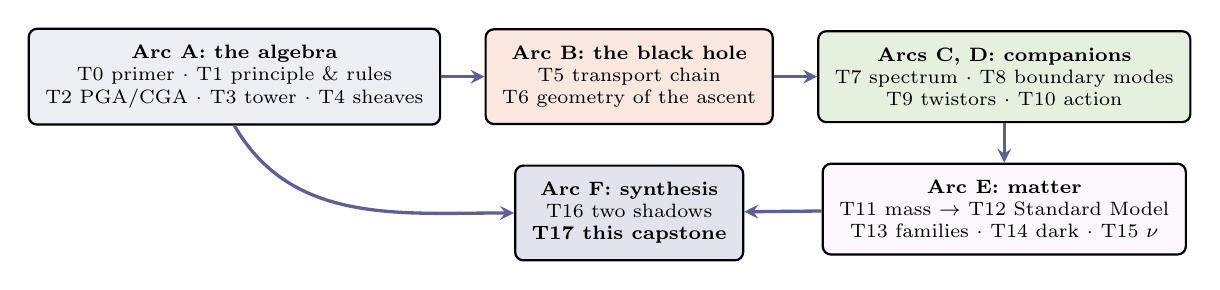
\begin{tikzpicture}[>=stealth, font=\scriptsize,
  arc/.style={draw, thick, rounded corners=3pt, inner sep=6pt, align=center},
  flow/.style={->, very thick, MidnightBlue!70}]
% Arc A
\node[arc, fill=MidnightBlue!8] (A) at (0,0)
  {\textbf{Arc A: the algebra}\\ T0 primer $\cdot$ T1 principle \& rules\\ T2 PGA/CGA $\cdot$ T3 tower $\cdot$ T4 sheaves};
% Arc B
\node[arc, fill=BrickRed!8, right=0.55 of A] (B)
  {\textbf{Arc B: the black hole}\\ T5 transport chain\\ T6 geometry of the ascent};
% Arcs C+D
\node[arc, fill=OliveGreen!10, right=0.55 of B] (CD)
  {\textbf{Arcs C, D: companions}\\ T7 spectrum $\cdot$ T8 boundary modes\\ T9 twistors $\cdot$ T10 action};
% Arc E
\node[arc, fill=Plum!8, below=0.5 of CD]  (E)
  {\textbf{Arc E: matter}\\ T11 mass $\to$ T12 Standard Model\\ T13 families $\cdot$ T14 dark $\cdot$ T15 $\nu$};
% Arc F
\node[arc, fill=MidnightBlue!12, below=0.5 of B] (Fk)
  {\textbf{Arc F: synthesis}\\ T16 two shadows\\ \textbf{T17 this capstone}};
\draw[flow] (A) -- (B);
\draw[flow] (B) -- (CD);
\draw[flow] (CD) -- (E);
\draw[flow] (E) -- (Fk);
\draw[flow] (A.south) to[out=-60, in=180] (Fk.west);
\end{tikzpicture}
\caption{The series map: six arcs, eighteen papers, read left to right. Each arrow is the principal direction of dependency between arcs (the algebra feeds everything; the black hole is the first application; the companions supply state, count, twistors, and action; matter builds on all four; the synthesis reads the whole). The fine-grained dependencies are declared per paper in each paper's imported Facts. Entry points for a new reader, in order: T1, then T5, then T16.}
\label{fig:map}
\end{figure}

Table \ref{tab:status} is the status table: each paper's current version, its payload in one line, its epistemic tier, its machine verification, and what remains. Two conventions govern it. The tier column records the paper's declared tier, with the per-result levels stated in the papers themselves; and the verification column counts the exact checks in the paper's deposited script, all of which pass, for a series total of 1762 checks across the sixteen companion scripts T1 to T16 (the primer's small script and this paper's audit are counted separately in Section \ref{sec:verification}). The page counts in the table are audited by that script against the compiled PDFs, and the check counts against the counts the companion papers record, or against a fresh run of every companion script when the audit is invoked that way.

\begingroup\small\setlength{\tabcolsep}{4pt}
\begin{longtable}{p{0.066\textwidth} p{0.045\textwidth} p{0.389\textwidth} p{0.09\textwidth} p{0.078\textwidth} p{0.224\textwidth}}
\toprule
\textbf{Paper} & \textbf{Ver.} & \textbf{Payload (one line)} & \textbf{Tier, status} & \textbf{Checks} & \textbf{What remains} \\
\midrule
\endhead
T0 & 1.0 & An introduction to geometric algebra: the primer companion, expository, every worked example machine-checked, closing with the toolkit of classical structural lemmas T1 imports, proved in full; the failure of division itself is deliberately left to T1 \cite{ButlerT0} & \hspace{0pt}companion; 16pp & 16 & Kept in step with the series' notation \\
T1 & 3.0 & The transport principle: the taxonomy N/P/C proved exhaustive; the no-go at the element with its cohomological form; total division at the point with minimality forced twice over; Rule 2 fusion with embedding-independent minimality; type P settled (no fourth rule); the mod-8 clock, the one-way door, and the six-step transport algorithm; the extension theorem (where the obstruction lies, and the commuting square) \cite{ButlerT1} & A; 51pp & 115 & The series' root; full-parabolic torsor class; conservation-of-obstruction conjecture (to T4's walls); the sign of $\nu^{2}$ \\
T2 & 1.0 & PGA completes minimally and uniquely to CGA, with the translator dictionary; the missing division is transported, not supplied by an inverse (the kinematic-singularity reading is this paper's remark in Section \ref{sec:thesis}, not T2's) \cite{ButlerT2} & A; 8pp & 20 & Sheaf-level degenerations of projective type (belongs to T4's methods) \\
T3 & 1.0 & Tower rigidity (the clock never ticks under Rule 1); one qubit per rung; Witt index as quantum capacity; the CAR limit at even transport charge \cite{ButlerT3} & A; 17pp & 31 & The odd-charge question (posed, not asserted) \\
T4 & 1.0 & The degeneration sheaf; one-sided completion; absolute conservation of degeneracy; tame wall induction and the infinite wall sequence; the exceptional algebra; the residue with the corrected twist $N^{*}\Sigma \cong L^{\otimes 2}$; two-sidedness of tame walls \cite{ButlerT4} & A; 50pp & 296 & Wall-class conjecture (coarse half proved); the Kasner-weights conjecture beyond the diagonal class, where the Schwarzschild weights are forced: the analytic dictionary with T6's admissibility class; the Kerr composite; the operator and state level at the wall; the variable-exponent weighted limit; edge regularity; the twisted completion \\
T5 & 1.0 & The six-step chain computed end to end for Schwarzschild, single-mode thermality, the bosonised photon sector, the count from named axioms, the Page envelope and eviction, and the explicit finite-mode model with the parity-protection lemma; the modular flow of the boundary modes as the $t$-line holonomy at $\beta_{\mathrm{H}} = 6\pi$, and (L$_E$) stated with its cost as stabiliser against tangent \cite{ButlerT5} & B; 77pp & 233 & Closure-completeness (the conjectural core inside axiom (L)); state selection (assigned to T7); the angular state on the exceptional set \\
T6 & 1.0 & Where division fails (unipotent ray, scale decoupling); the parallel ideal point with the $\Lambda \neq 0$ extension (norm $+\Lambda/3$, with its convention note); the weighted limit with values-level Levi boundary holonomy; Schwarzschild-de Sitter; the Kerr tests and the Cauchy-horizon derivative-level filtration; transport-level convergence along the tangential lines \cite{ButlerT6} & A/B; 31pp & 82 & Quantitative transport across the Cauchy horizon; billiard-invariant limit; ring blow-up; edge regularity; Carter's constant inside the gauge-theoretic formalism \\
T7 & 1.0 & The I-state with the pairing and the Fermi-Dirac symbol both forced by the KMS identity; the mode continuum; the Penrose homogeneity $-2s-2$ promoted to a stated result from T9's ordering shift; the helicity lift and greybody inheritance with the steps named; the finite mode space's exact edge and Planck identities (the $\ell_{P}^{2}/A$ correction) \cite{ButlerT7} & B; 21pp & 25 & Geometric modular action; the lift beyond assembly; the Kerr continuum; the $\ell_{P}^{2}/A$ correction per observable; the cosmological state; helicity counting per boundary mode (one channel or both, feeding T8's count) \\
T8 & 1.0 & The count with the internal cutoff's uniqueness; the epoch as the modular period (the flagged intrinsic-clock principle (IC)), converting to $\nu = 1/16\pi$ if and only if $N_{\mathrm{epoch}} = S_{\mathrm{BH}}$ (the convention throughout this survey: $\nu$ in the 1-nat convention, which is $1/(16\pi\ln 2)$ in T5's capacity convention, the one T8 gives physical content); the fuzzy transverse sphere by principality-from-indifference; the spreading law saturating the chaos bound; the no-attic route; the no-echo prediction against GWTC-4.0; the calibration factorised, $16\pi = 4\pi \times 4$, and the quarter examined down to the calibration residue $\kappa_{c} = 1/(4\ln 2)$ (a symbol T8 keeps distinct from the surface gravity $\kappa$) with no recount reaching it \cite{ButlerT8} & B/C; 23pp & 47 & Produce $\kappa_{c} = 1/(4\ln 2)$ from the boundary modes or refute (IC), the prediction depending on $\kappa_{c}$ alone and assigned to T8; the Kerr ring count; chaos beyond free-fermion spreading; the slice-to-epoch aggregation rule; catalogue currency \\
T9 & 1.0 & Twistors as ascended spinors (the Fock model); incidence is the completion's chart, term by term; local twistor transport as the spinor square root of the tractor connection; the palatial two-level architecture with the ordering shifts; the ordering-insensitivity theorem (the googly conjecture's algebraic half proved) \cite{ButlerT9} & A/B; 30pp & 69 & The analytic googly half; the quantised incidence relation \\
T10 & 1.0 & The Stelle-West vector made from the frozen point, $V = X - (3/\Lambda)I$; the curvature-squared presentation exists if and only if $\Lambda \neq 0$; the equations vacate what the completion fills; $w = -1$ on the Einstein region, registered with its condition; two kinds of action (gravity pre-metric); the acoustic no-go closed at the mixed level of its inputs; the fourth alternative, $N$ a parameter of the laws under the action as written, with the Henneaux-Teitelboim promotion that would make it initial data one of a known class of modifications of the action and a decision recorded open \cite{ButlerT10} & B; 36pp & 90 & The forcing half beyond the diagonal Kasner class; the dual wall; matter coupling at $\Sigma$ and the frozen point off the vacuum region (the condition on $w = -1$); the Kerr no-go; the smallness of $\Lambda$ behind the promotion decision \\
T11 & 1.0 & The mass-weight dictionary $m^{2} = -w(w+3)\langle I, I\rangle$, in dimension four $-w(w+3)\Lambda/3$, the de Sitter formula with $\Delta = -w$, nonnegative on real weights only for $w \in [-3, 0]$, every known massive particle at complex weight $-\tfrac32 \pm i\nu$; two-twistor mass as symplectic area; the exact join, the composite's grip on the frozen point as its de Sitter momentum, $m^{2} = 2|B_{\Lambda}|^{2} + \langle I_{\Lambda}, I_{\Lambda}\rangle C$ with the correction to the deformed bracket one term of coefficient $\Lambda/3$; the massless locus computed; the equivalence principle as a structural reading \cite{ButlerT11} & B; 24pp & 39 & The operator join and its ordering constants; a de Sitter chart adapted to the non-simple frozen point (shared with T6); the weight assignments (the hierarchy restated); the massless locus and the condensation seed; many-twistor composites \\
T12 & 2.0 & The Standard Model's algebra as automorphisms of $\C^{2}\otimes\C^{3}$ with the exact $\Z_{6}$ global form; the quark doublet as the cells and the singlet spectrum from the one-handed listing, with the lepton doublet, the common handedness, $\mathrm{Spin}(10)$ and $\sin^{2}\theta_{W} = 3/8$ under the declared hypothesis (S) of slot statistics; the one-loop run in closed form; the one number $N$ and the trichotomy with its fourth alternative; the partner sector quantified (no other tower contributes, complete multiplets inert, the one- and two-threshold criteria, the one-loop rows failing the proton condition and the supersymmetric row admissible at two loops); the slot/pair split as a Pati-Salam intermediate symmetry, with the thirteenth generator its broken $U(1)_{X}$, meeting at $3.4 \times 10^{16}$ GeV with the weak angle an input that the fermion masses fit without tuning when the second family's factor $3$ comes through mixing with the third by a grade-three direction, the route the series registers; the mass mechanism on the module (the frozen point insensitive to the slots, the doublet as the rung directions, the Yukawa pattern, the transported frozen point) and three no-go theorems on the Georgi-Jarlskog factor, every result of the mechanism that names a species under Hypothesis (S); the status proposition: the rung unit, $v/H \approx 10^{44}$, not derived and rescaling-invariant, so not kinematically an instance of $N$ \cite{ButlerT12} & B; 75pp & 243 & The rung unit and the rung component as a field; two loops at two thresholds; the pair-sector current in the mass mechanism; the orientation (with T14); the descent measure behind the promotion decision; Hypothesis (S) and the label-copy theorem; the intermediate scale; the coupling of the grade-three direction between the second and third families \\
T13 & 2.0 & Three families as the faces of a three-twistor composite, the bound imported at observation level and the identification a conjecture; condensation with the $\Lambda$-linear source; the thirteenth refutation, and democracy at structural level under the indifference premise and the Gram-square reading; Koide as a nullity condition for one member of the invariant family, the $2\pi/3$ phases Fourier coordinates carrying no hypothesis; the rank-one-plus-shift theorem and the classification of the displaced-Gaussian class, one clause by theorem and two at flagged preliminary computation; the terminal state as it stands (one open problem in three forms), the absolute scale's list of excluded routes closed by covariance; the $126$ doublet direction with its Georgi-Jarlskog Clebsch, the one direction carrying the factor on a single family, and the reversed order of operations; the lepton sector under T12's Hypothesis (S) \cite{ButlerT13} & C, declared; 28pp & 73 & The non-Gaussian completion; the Gram-square structure; the second-order breaking $S_{3} \to S_{2} \to 1$ and its modulus, now second to the two-term structure; the real structure of face space; the strong dressing; the absolute scale in three pieces and the weight pattern's coupling to the pair-sector current, or on T12's registered route the grade-three direction's coupling between the second and third families (with T12) \\
T14 & 2.0 & Eight towers, two sterile, six populated, five dark, five being the count of dark causal residues under Premise P3 and not the count of anything in the density ratio; exact stability by superselection; the mirror tower a copy of this one with one visible share to half a percent, so $\Omega_{\mathrm{dark}}/\Omega_{b} = 1 + 4.364$, the remainder symmetric and not derived; the unit-ball rule, one quantum of a common mass per unit ball of each tower's space on three premises of its own, returning the ratio as $(11\pi + 16)/(3\pi) = 5.364$, fitted, at observation level, with the floor $5.255$ for every thickness, and the composition it fixes passing the Bullet Cluster only with the odd towers' matter collisionless, a premise (T14b); the asymmetry inherited as initial data, with the fifteenth refutation a degree count and the dipole bound at its stated scope, and its strength $\epsilon$ a declared stance; the orientation as the arrow (the seventeenth refutation, a covariance argument on three premises, Hypothesis (S) among them); the radiation audit conditional on the deposit energy; the ceiling valued; infall by parallel boundary mode spaces under the fifth premise, mass-limited with the supermassive case open, the boundary modes holding entropy and not charge; the fork restated at its level, the bit read once on $(2,2)$ \cite{ButlerT14} & C, premises attacked; 74pp & 200 & Five open: the odd towers' content; the pre-descent theory (P1), with the reheating temperature and the deposit energy; the coupling rule; the burst dimming factor; the window. Closed in the negative: the partner question (no other tower contributes) \\
T14a & 1.0 & One dimension at a time (companion to T14): a single added generator doubles or complexifies the shadow by its sign, the mirror's algebra sitting on the anti-de Sitter translation bivectors; the rung's even subalgebra as the anti-de Sitter algebra, so the copy theorem's inputs live in the complexification; the frozen point's scale tractor and Stelle-West vector as the ascent's pair signed by $\Lambda$, the intermediate algebra of this world's own ascent and this tower's by the soldered residue; the transport constraining the frozen point only through its norm, so $\Lambda$ is undetermined within the series, its frame components gauge, its sign not a selector of the visible tower; the $\Lambda$ family a tame wall completed on both sides in the case the sheaf paper's conservation theorem excludes \cite{ButlerT14a} & C; 23pp & 86 & No prediction; the one observational input is the sign of $\Lambda$ \\
T14b & 1.0 & Simulating the dark towers (companion to T14): per unit of the mass gravity sees, the three-dimensional towers' cross-section is a length times the spacing of the sheets, the composite's size entering only through a logarithm; one multi-species code runs a Bullet-like merger, the assembly of a galaxy cluster and a model of the Milky Way in two readings of T14's composition; with the three-dimensional towers' matter colliding it fails the Bullet Cluster and the shapes of galaxy clusters, under either assignment of the shares; with it collisionless only the mirror's $18.6$ percent collides, the merger passes and the shapes are not excluded; the mirror in the Galaxy registered and not yet decidable \cite{ButlerT14b} & C; 36pp & 60 & The collisionless premise (the three-dimensional towers' couplings, which the series does not fix); the Galaxy test, which waits on a Gaia analysis with thicker dark disks and a bulge model with a disk-like dark component \\
T15 & 2.0 & The right-handed neutrino as the empty twistor at grade zero, its hypercharge computed as zero (the filled twistor is $e^{c}$ at $Y = -1$), with the proof that anomaly cancellation could not have fixed it; the sixteenth refutation (the deformed bracket's cosmological term cannot supply the mass); the seesaw with its Majorana scale a premise (M), valued at both ends of the Dirac mass, T12's Pati-Salam route selecting the bottom-like one; the light matrix exactly rank one at leading order, whatever $\alpha$ (the branch $\alpha \ll M_{3}$ is a separate premise, governing the breaking): inverted ordering excluded by rank rather than disfavoured by fit, and under the hierarchy premise (H) $\mnu \approx 0.059$ eV, $m_{\beta\beta}$ at $1.5$ or $3.7$ meV under the real-breaking assumption and in the hull $1.3$ to $3.9$ meV without it; the joint prediction with $w = -1$; leptogenesis suppressed under the reheating premise (R), with the $\delta_{CP}$ stance \cite{ButlerT15} & B/C; 22pp & 53 & The PMNS angles at second order; the two light masses and $\alpha$ (deciding (H)), and whether the branch survives on T12's Pati-Salam route; deriving $M$ (discharging (M), deciding (R)); the injected asymmetry from the descent's dynamics rather than the real-breaking assumption; dataset currency, every number refresh-at-submission by construction \\
T16 & 1.0 & The one relation's two presentations; Witt index as quantum capacity; every point a projective line of vacua and spacetime the manifold of such lines; the sorted overlap table; the third constant placed as the conversion constant between the charts, a conformal invariant below $\hbar$ and $G$; the $\nu = 4$ quadric where the incidence-line picture's exhaustiveness first fails; the laboratory's three postulates, one sourced, one half sourced, the third proved not a postulate, with the form of the law forced and $g = 2$ inherited; Born located with the additivity fragment isolated; the vote, on the indifference and recording premises and the flag's Hypothesis (S); experience as record-chain theorems under two premises, recording and supervenience, with Hypothesis (S) in the flow clause \cite{ButlerT16} & B/C; 31pp & 146 & Which capacity the state reads (half answered); the state-selection residue; thermal time plus state selection as the laboratory's remainder; emergent versus exact superselection; the additivity fragment; the primordial spectrum (assigned to this capstone) \\
T17 & 2.0 & This survey: the method, the status, the falsifiable claims, the measure, the directions, the thesis; with the audit script & survey; kept current & audit & Refreshed after every review round and every dataset move \\
\bottomrule
\caption{The status table. One row per series paper: the version printed on its title page, payload, declared tier and review status, exact-check count of the deposited verification script (all checks pass), and the declared remainder. The sixteen companion scripts carry 1762 checks in total; the primer's script and the audit script of Section \ref{sec:verification} are counted separately, and the audit checks every page count in this table against the compiled PDF and every check count against the count the companion paper records, or against a fresh run of its script.}
\label{tab:status}
\end{longtable}
\endgroup

One reading of the table is worth making explicit for the general reader. The series's claims are not uniformly strong, and the table is built so that the gradient is visible: the algebra arc is unconditional theorem-proving; the black-hole and companion arcs are exact mathematics assembled on named imports, with the physical inputs (a state, an epoch, two structural axioms) flagged and quantified; the matter arc derives structure outright but numbers only through flagged premises, and says so; and the synthesis is explicitly a reading of proved parts. What is uniform is the discipline: every claim carries its level, every level is printed, and everything computational is machine-checked. The table's "what remains" column is the programme's open directions in miniature, expanded in Section \ref{sec:directions}.

\section{The falsifiable claims}\label{sec:ledger}

The series' governing commitment to its reader is this: wherever the framework touches data, it registers a position in advance, in print, with the dataset named and the measurement that would refute it specified, and it keeps confronting that data as the record changes. The stances come in two strengths. A \emph{registered stance} is unconditional within the framework (row 2 carries the one condition T10 names and does not use): if the measurement goes the other way, a piece of the framework essential to its proofs is refuted with no parameter available to absorb the result. A \emph{conditional absence} is registered at the level of flagged premises: it says that if the framework's premises hold, a whole class of searches will return null forever, so that continued nulls are consistent with it and a single confirmed signal refutes the premises. Table \ref{tab:stances} gathers all twelve, with the confrontation column date-stamped August 2026 and refreshed at every revision of this paper, which is kept current.

\begingroup\small
\begin{longtable}{p{0.24\textwidth} p{0.05\textwidth} p{0.30\textwidth} p{0.28\textwidth}}
\toprule
\textbf{Stance} & \textbf{Paper} & \textbf{Dataset and current confrontation (2026-08)} & \textbf{Refutation condition} \\
\midrule
\endhead
\multicolumn{4}{l}{\emph{Registered stances (unconditional; a contrary measurement refutes structure used in the proofs)}}\\
\addlinespace[2pt]
1. No echoes: post-merger ringdown is the unmodified Kerr quasinormal spectrum & T8 & Gravitational-wave catalogues; through GWTC-4.0, four catalogues and four search methods report no significant echo train, and early tentative claims did not survive reanalysis \cite{GWTC4} & One statistically confirmed echo train at the Planck-structure delay \\
2. Dark energy cannot evolve: $w = -1$ exactly, at every epoch; registered with its one condition, that the frozen point admits a definition on a matter-filled region that keeps it parallel, which T10 names and does not use & T10 & DESI DR2 with CMB and supernovae; a three-to-four sigma preference for evolving $w$ is reported and contested (derivative-concentrated, prior-sensitive, internally tensioned); the stance does not rely on the dispute and states its exposure \cite{DESIDR2} & A confirmed detection of $w \neq -1$ at any epoch, with no parameter available to absorb it \\
3. The $\Z_{6}$ charge lattice: no fractionally charged colour singlet exists & T12 & PDG exotic-particle searches; consistent to date \cite{PDG} & One confirmed fractionally charged colour-singlet particle \\
4. $\mnu$ at the oscillation floor ($\approx 0.059$ eV) with normal ordering, the sum a prediction under T15's hierarchy premise (H) & T15 & Cosmological combinations; DESI DR2 with the CMB gives $< 0.064$ eV in $\Lambda$CDM \cite{DESIDR2}; the tightest current bound, $< 0.052$ eV at 95\% under a prior extending to zero, is Hou, Wang, Zhao and Zhang's, who read the excursion below the floor as an artefact of the prior and give $< 0.092$ eV with the physical floor imposed \cite{HouWangZhaoZhang2026} & Below: a physical-prior cosmological bound confirmed below the floor, or confirmed inverted ordering. Above: a sum determined meaningfully above the floor (near $0.075$ eV), or $m_{1}$ measured above a few meV, refutes the number while leaving normal ordering intact \\
5. The leptonic CP phase is trivial: $\delta_{CP} \in \{0, \pi\}$ & T15 & Joint long-baseline analyses currently allow CP conservation at three sigma under normal ordering and exclude it under inverted; the stance and the ordering prediction now depend on the same measurement & Confirmed CP violation in the leptonic sector under normal ordering \\
6. The internal prediction: $\nu = 1/16\pi$ in the 1-nat convention ($1/(16\pi\ln 2)$ in the capacity convention), equivalently one boundary-mode fermion per four Planck cells of horizon area per modular period ($N_{\mathrm{epoch}} = S_{\mathrm{BH}}$) & T8 & Internal: the geometry is closed at Schwarzschild (T6's tangential convergence), and the calibration residue $\kappa_{c} = 1/(4\ln 2)$ must be produced from the boundary modes themselves & A derivation of $\kappa_{c}$ from the boundary modes returning any other value, which refutes the intrinsic-clock premise (IC) \\
\addlinespace[4pt]
\multicolumn{4}{l}{\emph{Conditional absences (registered at the premises' level; continued nulls are consistent, one signal refutes)}}\\
\addlinespace[2pt]
7. Permanent direct-detection nulls: dark matter couples through gravity alone & T14 & All direct-detection programmes; null to date & Any confirmed dark-matter detection above the gravitational floor \\
8. No indirect dark-sector signals (annihilation or decay products) & T14 & Indirect-detection surveys; null to date & Any confirmed indirect signal \\
9. No dark radiation: $\Delta N_{\mathrm{eff}} \approx 0$, conditionally on the dark towers' open channels closing, which holds if the descent's deposit is no hotter than T14's estimate & T14 & CMB constraints \cite{Planck2018}; consistent & One confirmed massless dark species \\
10. No neutrinoless double-beta signal at next-generation sensitivity: $m_{\beta\beta}$ at $1.5$ or $3.7$ meV under Premise (H) and the real-breaking assumption, in the hull $1.3$ to $3.9$ meV without it & T15 & Double-beta programmes; the predicted values lie below the next generation's projected $10$ to $20$ meV band & A confirmed signal above the predicted window \\
11. Dimmed final evaporation bursts: the hole radiates into all six populated towers, five of them dark, so the visible burst is dimmed by the ratio of total to visible light degrees of freedom, of order the tower count if the towers are comparable & T14 & Primordial-black-hole burst searches; registered as a minor prediction, the towers' degree-of-freedom counts not derived & An undimmed final burst at the standard luminosity \\
12. No objective-collapse signature: no spontaneous-localisation noise, no gravitationally induced collapse & T16 & Collapse-model tests; null to date & One confirmed collapse signature, which ends the stance, the count of descent data, and the vote together \\
\bottomrule
\caption{The falsifiable claims: six registered stances and six conditional absences, each with its source paper, its dataset with the confrontation date-stamped August 2026, and its refutation condition. Rows 2 and 4 are jointly registered through shared datasets; rows 4 and 5 now depend on the same long-baseline measurement. Refreshed at every revision.}
\label{tab:stances}
\end{longtable}
\endgroup

Three structural remarks about the table. First, the stances are \emph{coupled}, deliberately: the dark-energy stance (row 2) and the neutrino sum (row 4) are jointly registered because the same survey combinations constrain both and because $w = -1$ removes the dark-energy parameter that could otherwise absorb a failing neutrino bound; and the ordering prediction and the phase stance (rows 4 and 5) have become one experimental question, since the current joint analysis excludes CP conservation under the ordering the framework already excludes. Whether the table should carry rows 4 and 5 merged into a single joint stance is an open presentational decision, recorded here rather than taken silently. Second, the table is \emph{asymmetric by design}: most rows are absences, and the framework has stated that absences are hard to confirm and easy to refute, which is the correct exposure for a framework whose distinctive claims are structural. The two positive numbers it does predict (the neutrino sum at the floor; the internal $1/16\pi$) are its two most exposed claims. Third, the table has \emph{already changed} since the stances were first registered: the echo confrontation has survived a fourth catalogue; the dark-energy preference has sharpened and remains contested; and the neutrino bound tightened below the floor under an unphysical prior and was called a prior artefact by its own analyses, which is the nearest thing to a confirmation of a stance that the record has yet offered. A framework that registers observational positions is worth more than one that does not; this table is where this one can be refuted.


\section{The measure: two numbers and one bit}\label{sec:measure}

Every quantitative freedom the framework retains has been counted into one small object, and this section states it, with the one scale the count does not yet place. What the framework's laws contain, as derived across the series, is \emph{initial data of the descent}, and the count across T12, T14, and T16 gives that data as two continuous numbers and one discrete bit. Beside it stands the weak scale: the Standard-Model paper's status proposition leaves the rung unit, $v/H \approx 10^{44}$ Hubble units, not derived, and either a second continuous number or an instance of the first, while its first successor problem records that the unit is rescaling-invariant and so not kinematically an instance of $N$; until it is placed, the count of two numbers is the count of the descent's data and not of every unexplained dimensionless constant \cite{ButlerT12}. The count's subject, dimensionless, is defined once the third constant is placed: the synthesis paper places $c$ as the conversion constant between the Witt chart and the metric chart, a conformal invariant below both $\hbar$ and $G$, and the three placements close the unit system, the exponent matrix of $(c, \hbar, G)$ over length, time and mass having determinant $-2$, so that every remaining constant is a dimensionless ratio \cite{ButlerT16}.

The first number is $N$, the number of the universe's boundary modes. The Standard Model paper proves the compression as monomial identities: the strength of gravity ($G\Lambda = 3N^{-2}$), the weakness of matter's self-gravity ($N^{-2}$), and the hierarchy of the weak scale ($\operatorname{Im} w = (m/M_{P})\,N$) are one number appearing three times, and the trichotomy classifies that number: not a coincidence (the Dirac reading is refuted by the $w = -1$ prediction), not a dynamical variable (by the frozen point's rigidity), and a datum of the descent, dated to the origin, on one condition the action paper now names: under the action as written $N$ is a parameter of the laws, constant on every solution and varying across the family of theories, and it is initial data only if the Stelle-West norm is promoted to a Lagrange-multiplier field whose constancy is an equation of motion, a decision the series records open with both branches stated \cite{ButlerT12, ButlerT10}; the companion T14a \cite{ButlerT14a} states the same freedom at the level of the algebra, the transport returning the rung and a canonical null frame and constraining the frozen point only through its norm $\Lambda/3$. The second number is $\epsilon$, the strength of the matter asymmetry, carried as a declared stance and not a classification: the dark-matter paper has the framework inherit its asymmetry as initial data of the descent rather than generate it, and its universality across the oriented towers is a theorem for the mirror and void for the odd residues \cite{ButlerT14}. The bit is the orientation of the planted Witt flag, and the seventeenth refutation argues it is a bit on three stated premises, CPT covariance of the derived gauge sector, the Standard-Model paper's Hypothesis (S), and the exhaustiveness of the trichotomy: CPT conjugation is a covariance of every kinematic structure the series checks, so on those premises the absolute orientation is underivable, and the framework locates what it cannot determine. That one bit is spent once and read twice: it is the matter-antimatter asymmetry's sign and it is the arrow of time, the same choice in two readings \cite{ButlerT14}, and the synthesis paper proves at $\Cl(1,3)$ level that the two readings cannot come apart, given the law \cite{ButlerT16}; on the two-time fork the bit exists but the arrow does not, so there it is read once.

The measure matters in two directions. Forward, it is what the programme leaves to cosmology: the last question of the framework is the physics of the first freezing, the dynamics that set $(N, \epsilon)$ and spent the bit, and that question belongs to cosmology (Section \ref{sec:thesis}). Backward, it is a constraint: because the count is fixed on its audited premises ($\epsilon$ a declared stance, the deposit energy a datum the framework does not fix, and, for the bit, the three premises of the seventeenth refutation, Hypothesis (S) among them), any proposal that requires fresh uncaused choices is not an open alternative within the framework, and the synthesis paper uses exactly this closure against dynamical collapse, which would produce one new uncaused bit per measurement event against a total of one on those premises \cite{ButlerT16}.

\section{The open directions}\label{sec:directions}

Ten research directions were open when the series began; it has since discharged, sharpened, or claimed most of them, and Table \ref{tab:directions} is the updated table: each direction, the paper it is now assigned to, and its state after the series' first pass. The table is the complement of Table \ref{tab:status}: what the series has not done, gathered as deliberately as what it has.

\begingroup\small
\begin{longtable}{p{0.30\textwidth} p{0.12\textwidth} p{0.48\textwidth}}
\toprule
\textbf{Direction} & \textbf{Assigned to} & \textbf{State after the series' first pass} \\
\midrule
\endhead
1. Sharpen the extensions & T1, T2, T4 & Largely discharged: the cohomological no-go with the torsor-mod-ideal formulation, representation-independent minimality with the exotic embeddings shown inert, and the PGA-to-CGA completion are now theorems. Remaining: the full-parabolic torsor class; sheaf-level degenerations of projective type. \\
2. The sheaf-theoretic programme & T4, T6 & Tameness done, the twist corrected, two-sidedness new. Remaining: the residue at sheaf level and the anisotropic case; the BKL-weights conjecture (the weighted anisotropic completion is the central construction; its analysis is closed at Schwarzschild, with T6's transport-level convergence along the tangential lines, so the $\nu$ prediction does not wait on it and depends on the calibration residue $\kappa_{c}$ alone); the wall-class conjecture (coarse half proved); the tractor and Fefferman-Graham dictionary beyond assembly. \\
3. Beyond the weighted limit & T6 & The limit proved for the AVTD class with the holonomy clause; Schwarzschild-de Sitter done. Remaining: the billiard-invariant version; edge regularity; the quantitative Cauchy-horizon transport theorem; the duality-monodromy conjecture over the ring. \\
4. Close the counting & T8, T6 & The epoch derived as the modular period on the flagged premise; the target reformulated integer-holographically ($N_{\mathrm{epoch}} = S_{\mathrm{BH}}$); both naive aggregations refuted exactly. The calibration is now factorised exactly, $16\pi = (\beta/r_{h})(A/S_{\mathrm{BH}})$, the quarter shown to be physics rather than a counting convention, and T6's tangential convergence closed at transport level, so the prediction does not wait on the geometry. Remaining: produce $\kappa_{c} = 1/(4\ln 2)$, one mode per Bekenstein-Mukhanov quantum per modular period, from the boundary modes, or refute (IC), the intrinsic-clock premise, assigned to T8; the Kerr ring count against Kerr entropy. \\
5. Select the state & T7 & The Fermi-Dirac symbol now derived from the KMS identity; uniqueness in the quasi-free class proved; the continuum carried through the CAR limit. Remaining: geometric modular action (the open problem); beyond quasi-free; the cosmological state of the descent. \\
6. Beyond the twistor kinematics & T9, T6 & The incidence question answered exactly; the googly conjecture's algebraic half proved (ordering-insensitivity of the anti-self-dual sector). Remaining: the analytic googly half; the quantised incidence relation; Carter's constant from the Killing-spinor identity; local twistors over the walls. \\
7. Exercise Rule 2 physically & T1 & Open. T1's extension theorem (where the obstruction lies, and the commuting square) supplies the algebra the direction needs: on every one-dimensional extension of an even-dimensional algebra exactly one sign obstructs, its ideals are copies of the base, and the opposite-sign repair is the Rule 1 ascent. What the series does not carry is a physical system in which that obstruction, exchange and repair are exhibited by a measured or standard structure. Remaining: such an instance, and what selects the sign of the adjoined generator, boost or rotation, conformal or spatial, the same bit the series' choice of $\Cl(2,4)$ rests on through T1's minimality argument. \\
8. Facing the universe & this paper & The stances gathered in Table \ref{tab:stances} and kept current. Remaining: the non-simple incidence chart (shared between T6 and T11); chaotic saturation beyond free-fermion spreading; and the smallness of $\Lambda$, now placed exactly: under the action as written $N$ is a parameter of the laws, so ``why this $\Lambda$'' is a question within one theory only if the Henneaux-Teitelboim promotion, one of a known class of modifications of the action, is adopted, a decision the series records open, and then a question for the descent measure no paper has begun; T14a \cite{ButlerT14a} gives the algebraic form of the same placement: the transport, run on the $\Lambda = 0$ wall, constrains the frozen point only through its norm, so neither the sign nor the magnitude of $\Lambda$ is produced by the ascent, and the sign does not select the visible tower. \\
9. Beyond the tower & T3, T4, T8 & The iteration question answered; the qubit ladder's algebraic reading supplied. Remaining: the odd-charge question; wall tameness for all couplings; the qubit ladder's physical reading, which is the $\nu$ question again. \\
10. The matter programme & T11-T15, T17 & Structure delivered at declared levels across six papers. The partner sector is quantified (no other tower contributes; the demand is split content; the one-loop rows fail the proton condition and the supersymmetric row is admissible at two loops), the slot/pair split supplies a Pati-Salam intermediate symmetry as the second route, on which the weak angle is an input that the fermion masses fit without tuning only if the second family's factor $3$ comes through mixing with the third by the grade-three direction, the Higgs doublet's representation and Yukawa pattern are derived from the rung directions, under Hypothesis (S) wherever a species is named, and three no-go theorems fix the shape of what is missing. Remaining, in the order the no-gos force: the two-term structure first, the coupling of the rung vector to the pair-sector current that the Georgi-Jarlskog factor needs and that neither the frozen point, the family structure nor the bracket supplies, on the registered route the grade-three direction's coupling between the second and third families; then the second-order breaking $S_{3} \to S_{2} \to 1$ acting on it (the CKM numbers and light masses); the rung unit and the rung component as a field; the intermediate scale; two loops at two thresholds; the dynamical potential behind the derived source term; the operator join with its ordering constants and the many-twistor grip (T11's successor problems); and the descent-sourced primordial spectrum against the measured index, the state being the first question, the programme item the synthesis paper assigns to this capstone itself and not begun. \\
\bottomrule
\caption{The open directions: the programme's ten research directions, updated against the series. Items are assigned to series papers; item 7 is T1's, and item 10's last entry (the primordial spectrum) is assigned to this capstone and not begun.}
\label{tab:directions}
\end{longtable}
\endgroup

\section{The successor programme: a theory of singularities}\label{sec:thesis}

\subsection{The thesis}

The programme's thesis can now be stated in one sentence, with every clause carried by a series paper rather than a promise: \emph{a singularity is not a place where physics ends but an interface where the description is forced up one level}, element to point \cite{ButlerT1}, metric to conformal \cite{ButlerT4, ButlerT6}, classical value to operator, c-number to ladder \cite{ButlerT3, ButlerT5}, by a completion that is minimal, unique, and one-way \cite{ButlerT1}. On this reading the singularity is a functor to be applied, not a pathology to be excised: its degeneration type determines its completion \cite{ButlerT1}; its rate of degeneration builds its exceptional geometry \cite{ButlerT4}; its blow-up weights are its Kasner exponents \cite{ButlerT6}; its boundary dynamics is a Levi excitation \cite{ButlerT6}; its field equations vacate exactly the directions its completion fills \cite{ButlerT10}; its modes are thermal at the temperature set by its own boost plane \cite{ButlerT5}; and its information deficit is a fixed, algebraically tracked projection rather than a loss \cite{ButlerT5}. The synthesis places the thesis inside a larger one: the completion functor acts on a spacetime already made, point by point, of the algebra's null elements, every point a projective line of quantum vacua, so a singularity is not where non-invertibility begins but where the vacuum family degenerates \cite{ButlerT16}.

Each clause is falsifiable in principle, and three tests are concrete enough to name. The BKL-weight identification can be tested in numerical relativity: Hubble-normalised holonomy should converge at the predicted power-law rate near generic singularities and fail to converge, in the predicted axis-rotating manner, in oscillatory ones. The mode count, repeated over the Kerr ring, must reproduce the known angular-momentum dependence of Kerr entropy or refute the counting (Table \ref{tab:directions}, item 4). And the conservation of degeneracy forbids any signature-change cosmology from smoothly eliminating its wall: the wall can be moved, never destroyed, a structural constraint on no-boundary-type proposals checkable model by model \cite{ButlerT4}.

\subsection{Other applications, and the successor programme}

The pattern (a classical description divides by zero; a completed description resolves it at the level of a larger space; the divergence is confined to a scale while a shape survives) is not specific to black holes. Cosmology is its principal successor, on four counts: isotropic big-bang singularities are conformally far tamer than black-hole interiors, so the tame sheaf theory applies to the early universe more directly than to the objects it was built for; the shadow wall gives the interface between aeons in cyclic proposals a precise algebraic description; signature change is already inside the formalism, as the clash of ascents at Euclidean-Lorentzian walls; and the programme's own dating places the descent at the origin, reading the big bang as the freezing itself, with $\Lambda$ the residue of that origin, $N$ the number of boundary modes it opened, and the dynamics of the first freezing left to cosmology as the framework's last question \cite{ButlerT12, ButlerT14}. Outside gravity, the oldest instance of the pattern is optics: a caustic is a locus where the ray description divides by zero, and its resolution by wave optics, the Airy function replacing the infinity and the Maslov index recording a monodromy, is a small instance of the transport principle. Analogue-gravity systems, whose effective acoustic metrics degenerate at sonic horizons, inherit the results wholesale. And one application is resolutely practical: engineering and robotics already compute in projective and conformal geometric algebra, where kinematic singularities are corank drops of a Jacobian, and the completion prescription (adjoin the dying direction, re-metrised by its rate of degeneration) is an algorithm that may yield principled regularisations where current practice damps singularities ad hoc \cite{ButlerT2}.


\section{Machine verification}\label{sec:verification}

A survey proves little and quotes much, so its script has a different task from the companion scripts': it is a \emph{consistency audit}. The script \texttt{verify\_T17.py} \cite{ButlerVerifyT17} imports the series' shared exact-arithmetic library \texttt{GA.py}; exact rationals, integers, and certified interval brackets throughout, no floating point anywhere; seventy-five checks when every companion file is present, all passing, in six parts. What it audits is stated exactly. For each of the seventeen companion papers T0 to T16 it opens the companion's compiled PDF and reads the page count from the file's own page tree, and it reads the companion's check count from the count the companion paper records in the version block of its source (or, when invoked with \texttt{--run-siblings}, from a fresh run of the companion script, counting the PASS lines it prints), and compares both with the status table and with the script's own recorded values; a companion file that is absent is reported as skipped, never as passing. It parses this paper's four tables from the source and counts their rows. It recomputes the physical numbers the paper quotes. Because this paper is kept current, the audit is also its refresh mechanism: when a review round changes a companion's page or check count, the corresponding check fails until this survey is regenerated, so a stale quotation is a reported error rather than a silent one.

\emph{Part A: the series' counts} (forty-seven checks). The paper inventory (eighteen papers, numbered consecutively, the identifiers 0 through 17 read from the file stems); the status table parsed and compared with the recorded page and check counts; the series total of 1762 computed from the recorded counts and compared with every place the body prints it; seventeen page counts read from the companion PDFs; seventeen check counts read from the companion papers' records or scripts; the version column read against the version printed on the title page of each of the twenty papers in the table; the refutation table's rows covering the ordinals 1 to 17 exactly once, each row naming its carrying paper; the stance table's six-plus-six, numbered in order; the ten open directions, each assigned; the measure's cardinality, two numbers and one bit, at each site the paper states it; and this paper's own compile log, which must carry no float-overflow warning (every table here is a breakable longtable) and no undefined reference.

\emph{Part B: the black-hole numbers}, as exact monomials in $\pi$ and $M$: $\beta = 8\pi M$ with $\beta/2\pi = 4M$; the epoch volume $V = \beta^{2} = 64\pi^{2}M^{2}$; the equivalence $\nu = 1/16\pi \iff N_{\mathrm{epoch}} = \nu V = 4\pi M^{2} = S_{\mathrm{BH}}$; and the naive count's overshoot by exactly $16\pi$, the horizon-area coefficient.

\emph{Part C: the dark count.} The sterile residues computed as the fixed points of $r \mapsto -r$ mod 8 (exactly $\{0, 4\}$); the count of five dark causal residues; and the ratio arithmetic T14 states, with five entering none of it: the symmetric remainder $4.364 = 5.364 - 1$ once the mirror's one share is removed; that remainder as $\Omega h^{2} = 4.364 \times 0.02237$, inside $0.0976 \pm 0.0012$; and the mirror's share of the dark density, $1/5.364$, between $18.6$ and $18.7$ percent.

\emph{Part D: the matter numbers.} The two exact one-loop rationals ($78761/379488$ and $6539/28320$) bracketed to four decimals, with the over-twenty-times-closer inequality against the measured angle; the integer bracket $2^{398} < 10^{120} < 2^{399}$; the hypercharge quadratic's roots, sum, and product; $3/8$ as the exact trace ratio; the frozen-point norm $\ip{I}{I} = \Lambda/3$ as a rational-function identity in formal $\Lambda$, and the dictionary's sign, $m^{2} = -w(w+3)\Lambda/3$, positive at the midpoint $w = -\tfrac32$ of the real interval $[-3, 0]$ and negative at $w = 1$ outside it, with the principal-series form $m^{2} = (\nu^{2} + \tfrac94)\Lambda/3$ at $w = -\tfrac32 + i\nu$ as a polynomial identity in formal $\nu$; and the compression identity $G\Lambda N^{2} = 3$.

\emph{Part E: the neutrino numbers}, by certified interval arithmetic (integer-square-root brackets on the mass-squared splittings): the normal-ordering floor confined to $(0.057, 0.061)$ eV and containing the predicted $0.059$; the $0.052$ eV zero-extending-prior bound strictly below the floor; the $0.092$ eV physical-prior bound above it; the inverted-ordering requirement above $0.097$ eV; the two $m_{\beta\beta}$ values recomputed from the splittings and the mixing brackets under the hierarchy premise and real breaking, bracketing $1.5$ and $3.7$ meV inside the hull $1.3$ to $3.9$ meV and below next-generation sensitivity; the quoted Koide value inside $2/3 \pm 10^{-5}$; and the Cabibbo bracket containing $0.225$.

\emph{Part F: the capacity identities.} The Witt index of Lorentzian signature (one); the increment identity on an exhaustive grid; and the ascended capacity three, equal on both sides of the chart.

What the audit does not and cannot check is what no script can: whether the source papers' proofs are correct (their own scripts and Leon's review carry that), whether the tiers are correctly assigned, whether the payload and remainder cells describe their papers faithfully, and whether the method section's claims about method are true of the practice. The audit guarantees a weaker and more useful thing: that the page and check counts this survey quotes are the companions' own, that its tables agree with one another, and that the physical numbers it repeats recompute.

\section{Position in the series}\label{sec:position}

This paper is T17 of the series. \emph{It relies on all seventeen predecessors,} T0 \cite{ButlerT0} through T16 \cite{ButlerT16}: the primer T0 \cite{ButlerT0}; the algebra arc, T1 \cite{ButlerT1}, T2 \cite{ButlerT2}, T3 \cite{ButlerT3} and T4 \cite{ButlerT4}; the black-hole arc, T5 \cite{ButlerT5} and T6 \cite{ButlerT6}; the quantum companions T7 \cite{ButlerT7} and T8 \cite{ButlerT8}; the identification arc, T9 \cite{ButlerT9} and T10 \cite{ButlerT10}; the matter arc, T11 \cite{ButlerT11}, T12 \cite{ButlerT12}, T13 \cite{ButlerT13}, T14 \cite{ButlerT14} with its companions T14a \cite{ButlerT14a} and T14b \cite{ButlerT14b}, and T15 \cite{ButlerT15}; and the synthesis T16 \cite{ButlerT16}. Every row of the status table, every entry of the refutation table and every stance is one of those papers' results, quoted at the level the paper declares.

\emph{Papers that rely on this one:} none depends on its results, since it proves nothing the companions use. T2 \cite{ButlerT2}, T15 \cite{ButlerT15} and T16 \cite{ButlerT16} cite it for the numbering of the stances and for the claim table.


\begin{thebibliography}{99}

\bibitem{ButlerT0}
L.~Butler,
\emph{An Introduction to Geometric Algebra: A Primer for the Transport Papers},
Transport Papers T0 (2026), doi:\href{https://doi.org/10.5281/zenodo.22714501}{10.5281/zenodo.22714501}.

\bibitem{ButlerT1}
L.~Butler,
\emph{The Transport Principle: Total Division in Clifford Algebras via Minimal Completion},
Transport Papers T1 (2026), doi:\href{https://doi.org/10.5281/zenodo.21743863}{10.5281/zenodo.21743863}.

\bibitem{ButlerT2}
L.~Butler,
\emph{Projective Completes to Conformal: The Minimal Nondegenerate Completion of a Degenerate Clifford Algebra, and Where PGA's Missing Division Goes},
Transport Papers T2 (2026), doi:\href{https://doi.org/10.5281/zenodo.22714886}{10.5281/zenodo.22714886}.

\bibitem{ButlerT3}
L.~Butler,
\emph{The Tower and the CAR Limit: Iterated Transport, the Frozen Clock, and Second Quantisation},
Transport Papers T3 (2026), doi:\href{https://doi.org/10.5281/zenodo.22721556}{10.5281/zenodo.22721556}.

\bibitem{ButlerT4}
L.~Butler,
\emph{Clifford Sheaves over Degenerate Metrics: Nilpotent Ideals, One-Sided Completion, and the Exceptional Algebra},
Transport Papers T4 (2026), doi:\href{https://doi.org/10.5281/zenodo.22721669}{10.5281/zenodo.22721669}.

\bibitem{ButlerT5}
L.~Butler,
\emph{Division by Zero at the Gravitational Singularity: The Transport Principle Applied to the Black Hole, and the Information Paradox as a Category Error},
Transport Papers T5 (2026), doi:\href{https://doi.org/10.5281/zenodo.22721790}{10.5281/zenodo.22721790}.

\bibitem{ButlerT6}
L.~Butler,
\emph{The Geometry of the Black-Hole Interior: Where Division Fails, the Weighted Limit, and the Kerr Tests},
Transport Papers T6 (2026), doi:\href{https://doi.org/10.5281/zenodo.22721990}{10.5281/zenodo.22721990}.

\bibitem{ButlerT7}
L.~Butler,
\emph{Hawking Radiation from the Ledger: State, Continuum, Lift, and the Finite-Ledger Seam},
Transport Papers T7 (2026), doi:\href{https://doi.org/10.5281/zenodo.22722121}{10.5281/zenodo.22722121}.

\bibitem{ButlerT8}
L.~Butler,
\emph{Black-Hole Entropy and Scrambling: The Singularity Ledger and the No-Echo Prediction},
Transport Papers T8 (2026), doi:\href{https://doi.org/10.5281/zenodo.22722176}{10.5281/zenodo.22722176}.

\bibitem{ButlerT9}
L.~Butler,
\emph{The Twistor Correspondence: Ascended Spinors, Incidence, and the Palatial Bridge},
Transport Papers T9 (2026), doi:\href{https://doi.org/10.5281/zenodo.22722290}{10.5281/zenodo.22722290}.

\bibitem{ButlerT10}
L.~Butler,
\emph{Dark Energy and the Action of Gravity: MacDowell-Mansouri, the Frozen Point, and One Way to Grip},
Transport Papers T10 (2026), doi:\href{https://doi.org/10.5281/zenodo.22722496}{10.5281/zenodo.22722496}.

\bibitem{ButlerT11}
L.~Butler,
\emph{The Origin of Mass: The Weight Dictionary and the Exact Join},
Transport Papers T11 (2026), doi:\href{https://doi.org/10.5281/zenodo.22722565}{10.5281/zenodo.22722565}.

\bibitem{ButlerT12}
L.~Butler,
\emph{The Standard Model from the Minimal Massive Composite},
Transport Papers T12 (2026), doi:\href{https://doi.org/10.5281/zenodo.22722669}{10.5281/zenodo.22722669}.

\bibitem{ButlerT13}
L.~Butler,
\emph{Quark and Lepton Families: Condensation, Democracy, and the Koide Relation},
Transport Papers T13 (2026), doi:\href{https://doi.org/10.5281/zenodo.22722845}{10.5281/zenodo.22722845}.

\bibitem{ButlerT14}
L.~Butler,
\emph{Dark Matter and the Arrow of Time: The Five Dark Towers},
Transport Papers T14 (2026), doi:\href{https://doi.org/10.5281/zenodo.22722953}{10.5281/zenodo.22722953}.

\bibitem{ButlerT14a}
L.~Butler,
\emph{One Dimension at a Time: The Odd Extensions of the Oriented Towers},
Transport Papers T14a (2026), doi:\href{https://doi.org/10.5281/zenodo.23232104}{10.5281/zenodo.23232104}.

\bibitem{ButlerT14b}
L.~Butler,
\emph{Simulating the Dark Towers: Methods, Assumptions and Tests of the Unit-Ball Composition},
Transport Papers T14b (2026), doi:\href{https://doi.org/10.5281/zenodo.23234576}{10.5281/zenodo.23234576}, deposited with its simulation code, run outputs and films; the films are also on YouTube, ``Galaxy clusters in collision'' (\url{https://www.youtube.com/watch?v=0SvmSwInN0c}) and ``The Bullet moment'' (\url{https://www.youtube.com/watch?v=KQnZUVR7bCk}).

\bibitem{ButlerT15}
L.~Butler,
\emph{Neutrino Masses: The Empty Twistor, the Seesaw Scale, and the Bet at the Floor},
Transport Papers T15 (2026), doi:\href{https://doi.org/10.5281/zenodo.22723070}{10.5281/zenodo.22723070}.

\bibitem{ButlerT16}
L.~Butler,
\emph{Quantum Mechanics and General Relativity from One Relation: The Two Shadows and the Laboratory},
Transport Papers T16 (2026), doi:\href{https://doi.org/10.5281/zenodo.22723212}{10.5281/zenodo.22723212}.

\bibitem{Popper1963}
K.~R. Popper,
\emph{Conjectures and Refutations: The Growth of Scientific Knowledge},
Routledge (1963).

\bibitem{Lakatos1978}
I.~Lakatos,
\emph{The Methodology of Scientific Research Programmes},
Cambridge University Press (1978).

\bibitem{GWTC4}
LIGO Scientific Collaboration, Virgo Collaboration, and KAGRA Collaboration,
\emph{GWTC-4.0: an updated catalog of gravitational-wave transients},
(2025--2026). % Refresh at submission.

\bibitem{DESIDR2}
DESI Collaboration,
\emph{DESI DR2: baryon acoustic oscillations and constraints on dark energy and neutrino mass},
(2025--2026). % Refresh at submission.

\bibitem{HouWangZhaoZhang2026}
H.~Hou, S.~Wang, Z.-C.~Zhao, and X.~Zhang,
\emph{Constraints on the sum of neutrino masses from ACT DR6 and DESI DR2 considering isocurvature initial conditions},
preprint arXiv:2606.17994 (2026). % Refresh at submission.

\bibitem{PDG}
Particle Data Group,
\emph{Review of Particle Physics},
current edition. % Refresh at submission.

\bibitem{Planck2018}
Planck Collaboration,
\emph{Planck 2018 results. VI. Cosmological parameters},
Astron. Astrophys. \textbf{641} (2020), A6.

\bibitem{ButlerVerifyT17}
L.~Butler,
\emph{verify\_T17.py: the consistency audit for the Transport Programme capstone},
Python script, deposited with this paper alongside the shared library GA.py (2026).

\end{thebibliography}

\end{document}
